\chapter{Design}

\section{Overall System Design}

\subsection{Short description of the main parts of the system}

\begin{itemize}
    \item Media Inventory Database
    \begin{itemize}
        \item General Interface
        \item Adding Records
        \item Displaying Records
        \item Searching Records
        \item Editing Records
        \item Deleting Records
    \end{itemize}
\end{itemize}

General Interface
\begin{itemize}
    \item The user will be presented with a box whereby he/she will enter a password. This password will be the same for all users who have access to the system.
    \item Once logged in, the user will be confronted with an interface consisting of a series of menu options. These options will be "Add Record", "Display Records", "Search Records", "Edit Record", "Delete Record" and "Change Password".
    \item When the "Change Password" button has been clicked, the user will be taking to a box where they will be required to enter the previous password, then enter a new password twice.
    \item Clicking on the "Add Record" button will take the user to an interface where they will be required to select the type of record they wish to enter.
    \begin{itemize}
        \item Clicking the "Add Loan" button will present an interface to the user where they will have a choice of selecting an existing customer specific loan or creating a new customer specific loan.
        \item Selecting the "Add PAT Test" button will present the user with an interface to choose a PAT test date or to create a new PAT test date.
    \end{itemize}
    \item Clicking on the "Display Records" button will send the user to an interface where they will have to select the table from which table they wish to see the records.
    \item Clicking on the "Edit Records" button will send the user to an interface where they will have to select the table from which they want to edit a record.
    \item Clicking on the "Delete Records" button will send the user to an interface where they will have to select the table from which they wish to delete a record.
\end{itemize}

Adding Information
\begin{itemize}
    \item The system will present the user with a drop down menu from which the user will have to choose an option for which to enter information. After selecting the option, the user will then be presented with a group of data to add to the new record. If any of these options require the user to enter data relating to another table within the database, they will be presented with a drop down menu and will be required to select an option before they record can be created.
    \item Once all the required data fields have been complete, the system will add a unique identifier to the record of information and save in to the database
\end{itemize}

\newpage

Displaying Records
\begin{itemize}
    \item The system will present the user with an interface with a drop down menu, where they will have to select the database  table from which they wan to view the data.
    \item Once the table has been selected, the user will then be presented with a view table that will display all the records within that database  table. They can then choose to sort this information into ascending or descending order by selecting any row for which to sort it by.
\end{itemize}

Editing Records
\begin{itemize}
    \item The system will bring up a user interface that will present a drop down menu where the user will have to select a database table from which they wish to edit a record.
    \item Once a table has been selected, the user will then be confronted with a user interface which will display all the records within that table and then prompt the user to select the record they would like to edit, by enter the unique identifier of this record.
    \item When the record has been selected, the user will be presented with an interface similar to the one where the user enters a new record, but the fields already contain the information. The user will then have to update which field of information to update.
    \item Once data has been updated and a "Done" button has been clicked, the user will then be asked to confirm the updates.
    \item When the updates have been confirmed, the system replace the old record with the new updated record.
\end{itemize}

Deleting Records
\begin{itemize}
    \item The system will present the user with an interface containing a drop down menu where they will have to select a database table from which they wish to delete a record.
    \item After the database table has been selected, the user will be presented with a view table showing all the records within the database table. Underneath the view table will be a prompt, asking the user for the unique identifier of the record they wish to delete.
    \newpage
    \item When the user has selected the record they wish to delete, they will have to confirm this by entering the system password.
    \item The system will then remove the record from the database permanently.
\end{itemize}

\newpage

\subsection{System flowcharts showing an overview of the complete system}

\begin{figure}[H]
    \begin{center}
        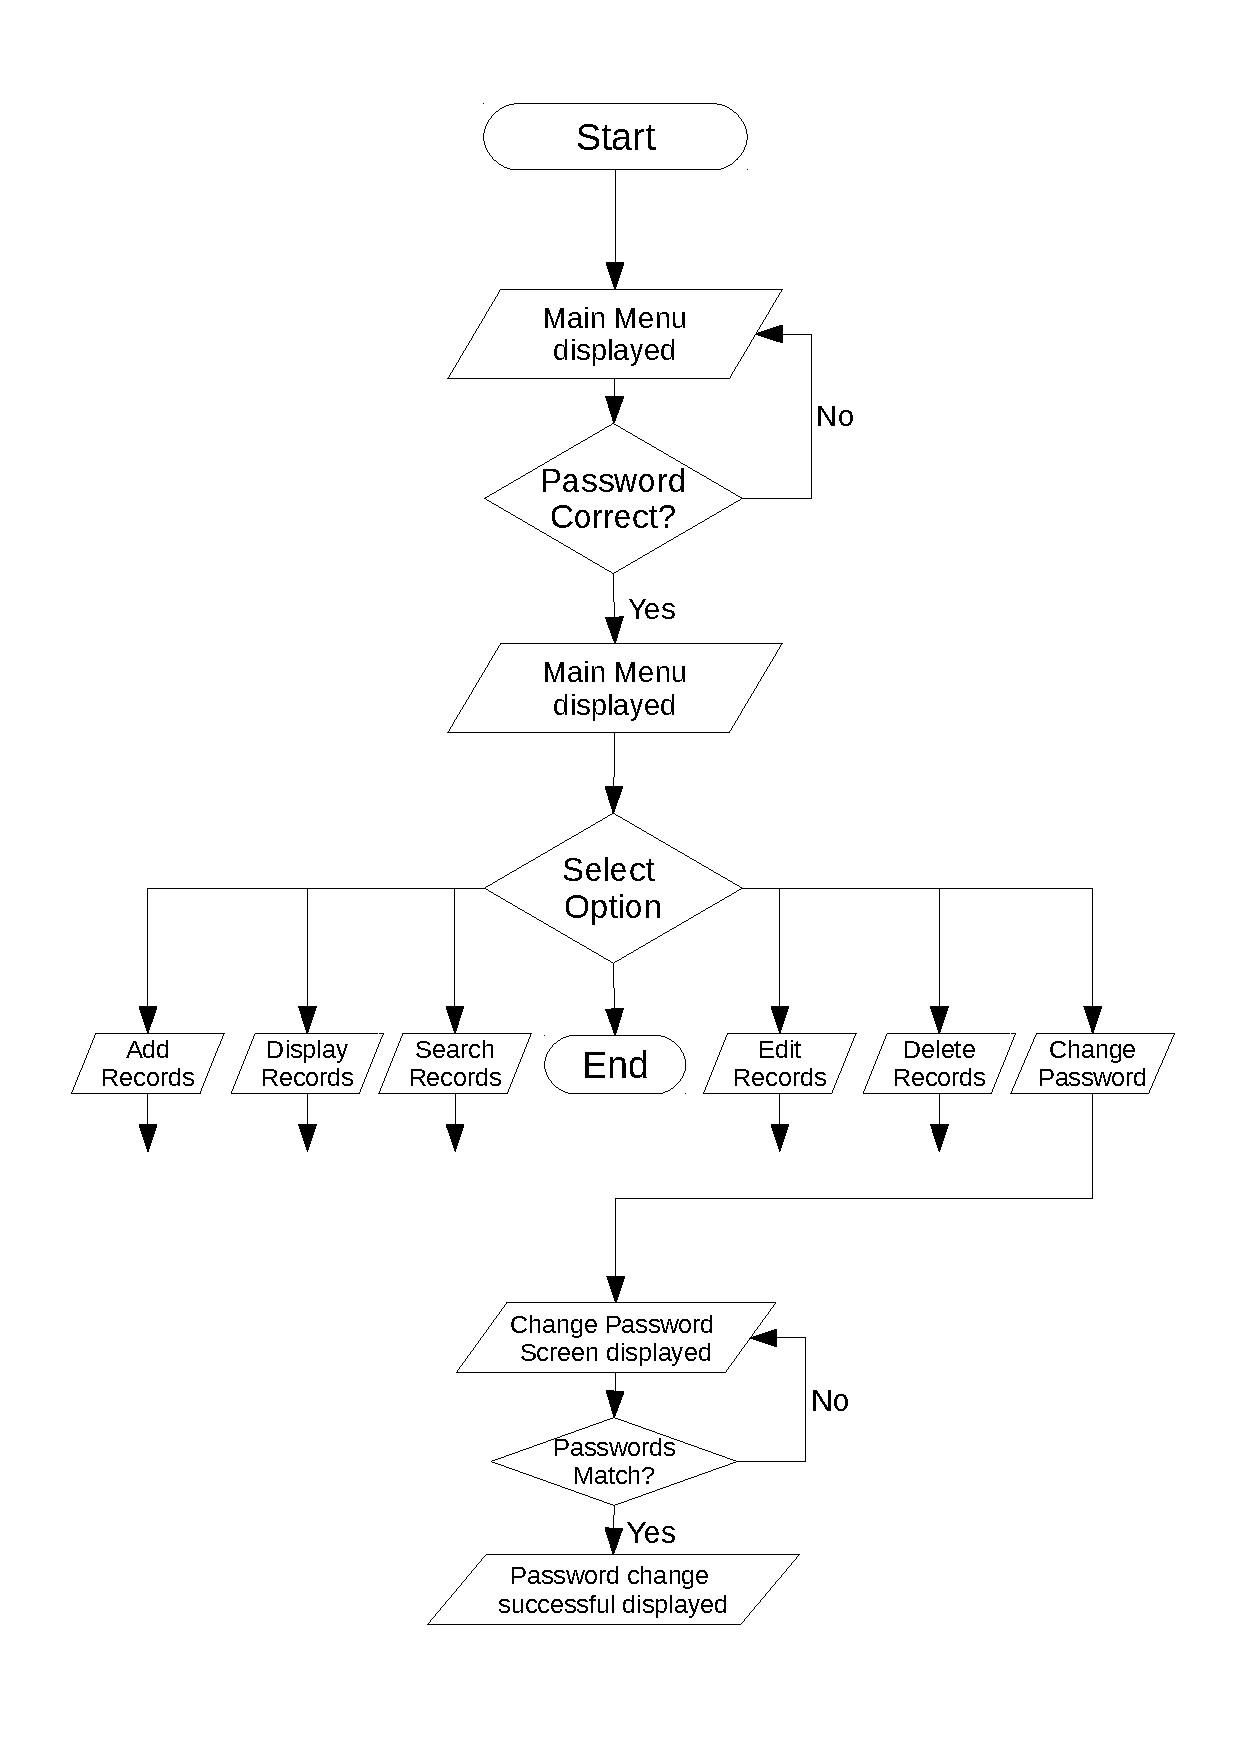
\includegraphics[width=355px]{./Design/system_flowcharts/PDFs/main_system_flowchart.pdf}
    \end{center}
    \caption{Main System Flowchart.} \label{fig:print_function_result}
\end{figure}

\begin{figure}[H]
    \begin{center}
        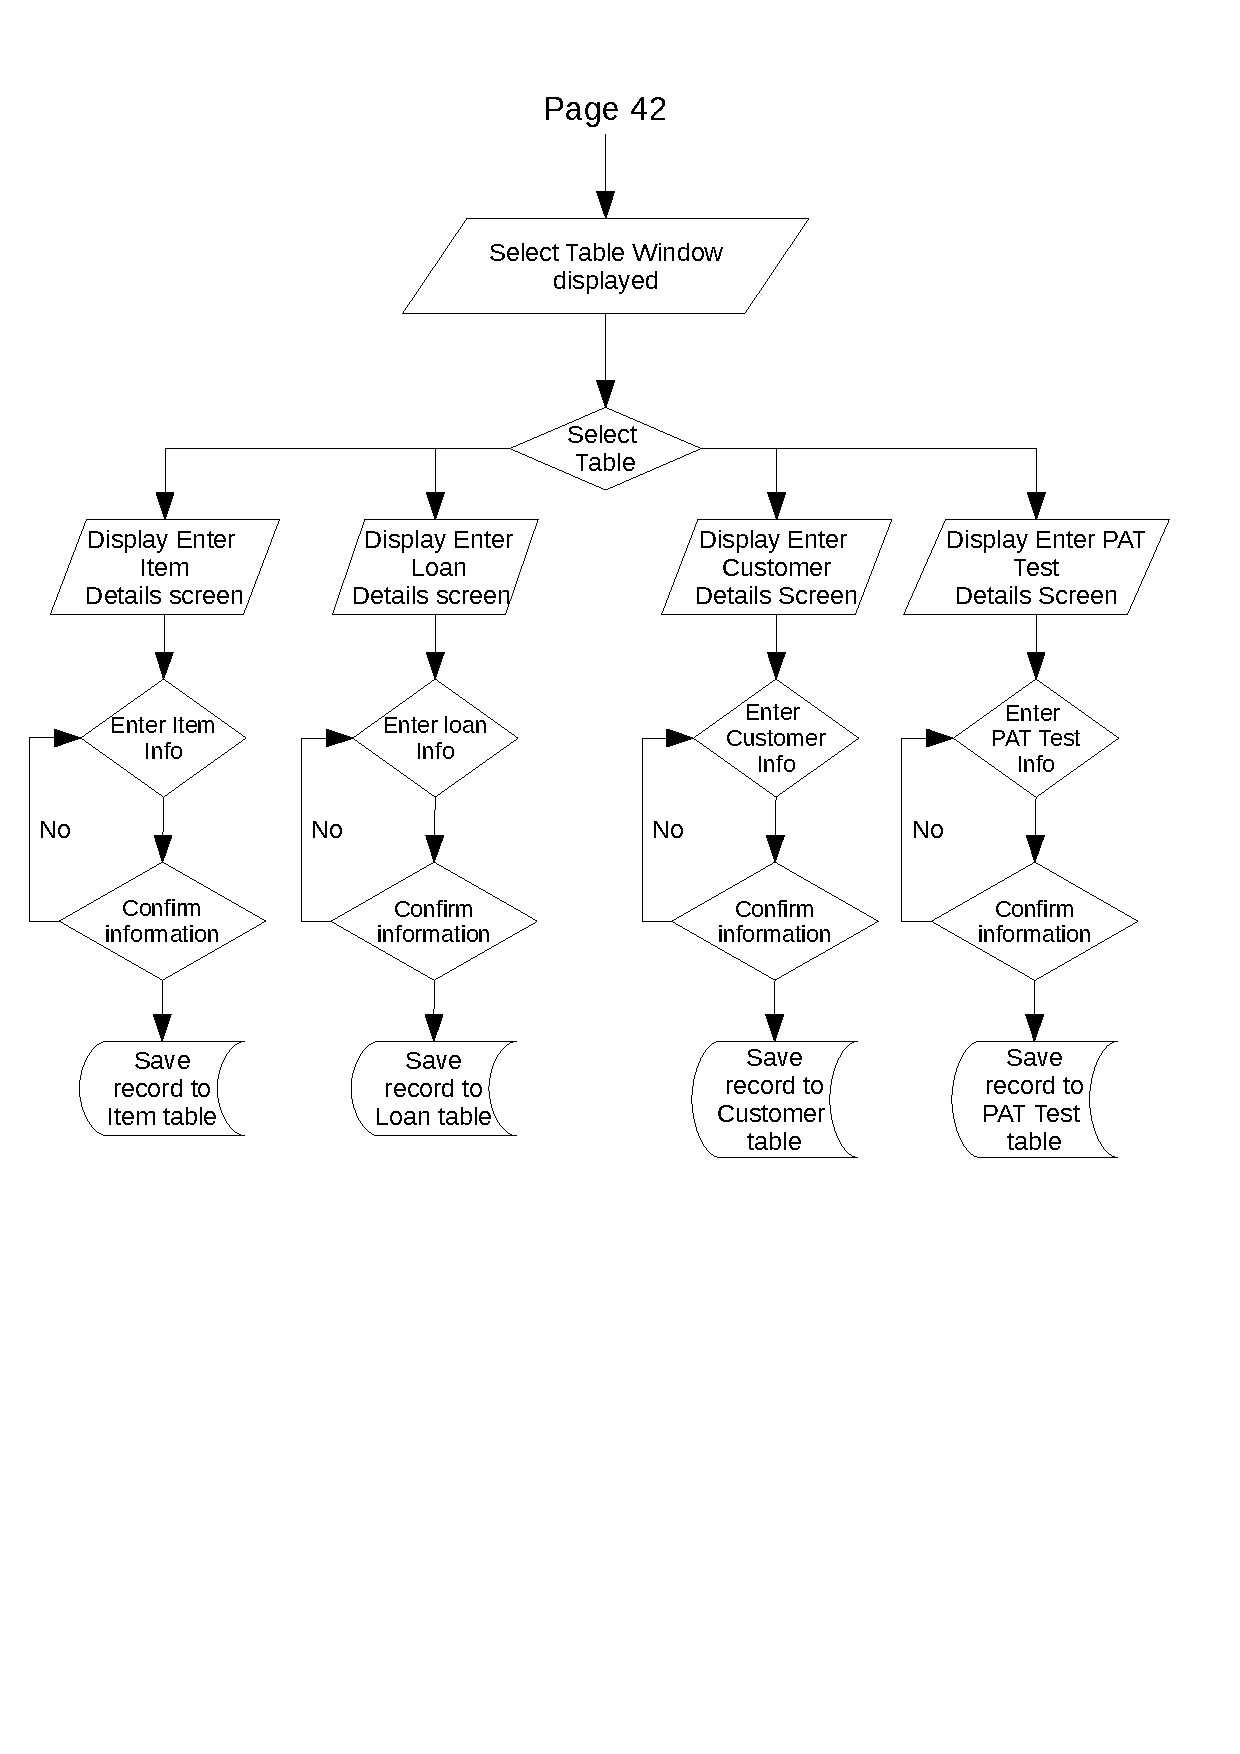
\includegraphics[width=355px]{./Design/system_flowcharts/PDFs/add_records_flowchart.pdf}
    \end{center}
    \caption{Add Records Flowchart.} \label{fig:print_function_result}
\end{figure}

\begin{figure}[H]
    \begin{center}
        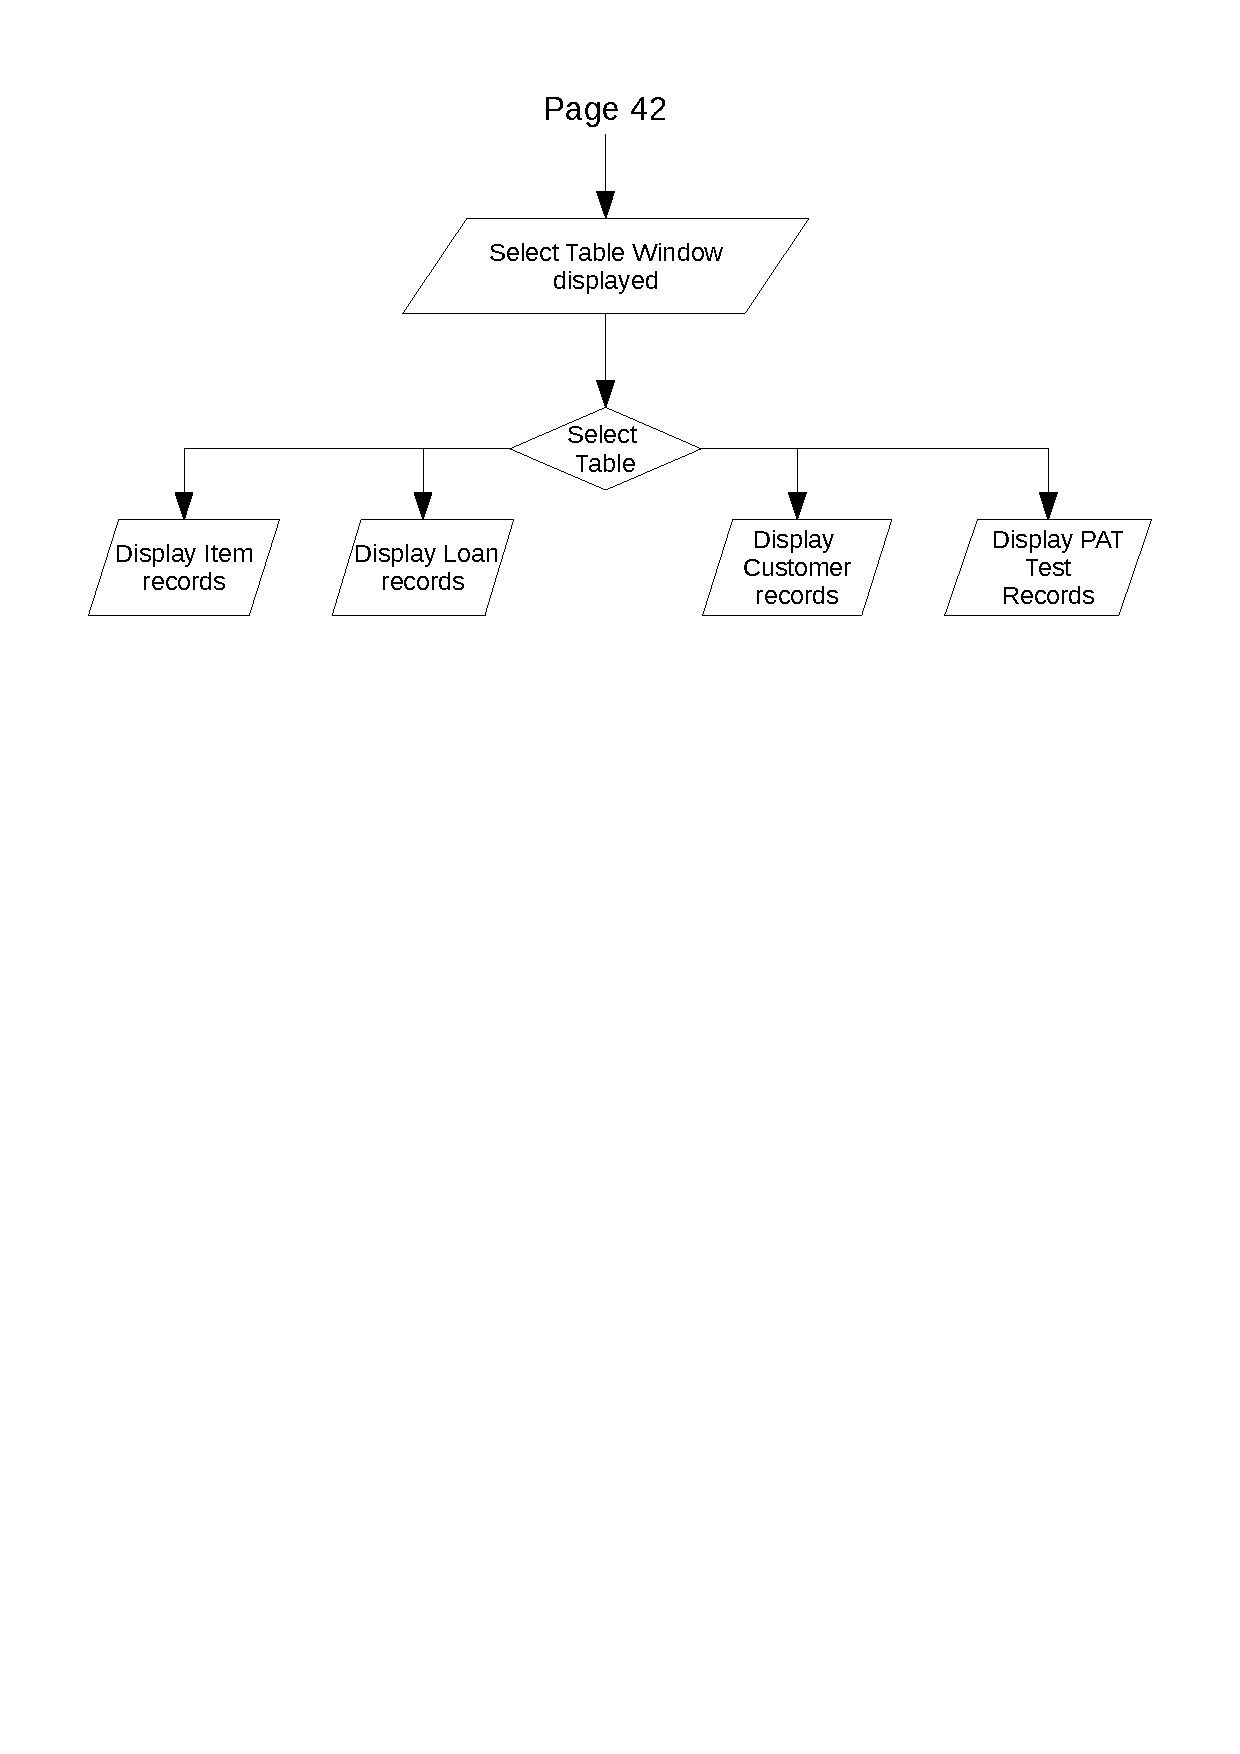
\includegraphics[width=355px]{./Design/system_flowcharts/PDFs/display_records_flowchart.pdf}
    \end{center}
    \caption{Display Records Flowchart.} \label{fig:print_function_result}
\end{figure}

\begin{figure}[H]
    \begin{center}
        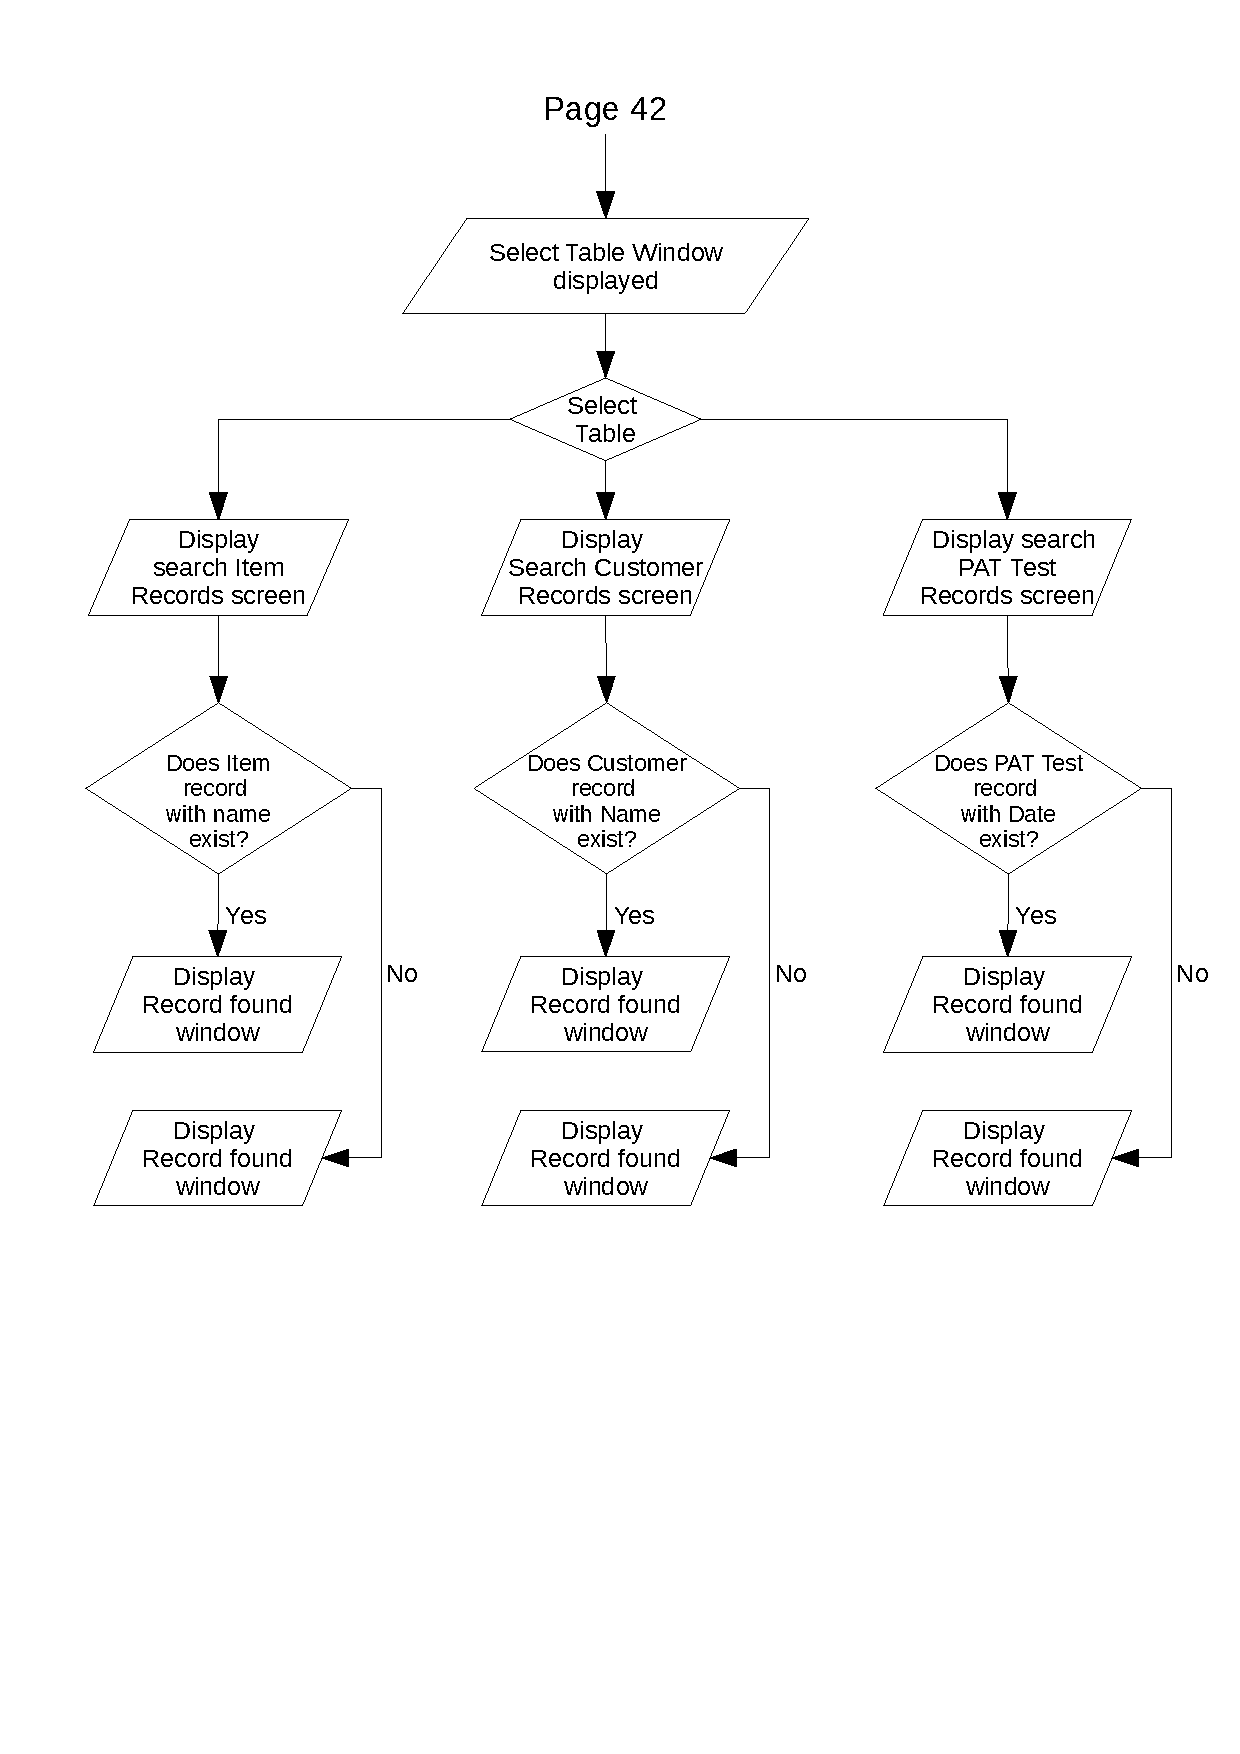
\includegraphics[width=355px]{./Design/system_flowcharts/PDFs/search_records_flowchart.pdf}
    \end{center}
    \caption{Search Records Flowchart.} \label{fig:print_function_result}
\end{figure}

\begin{figure}[H]
    \begin{center}
        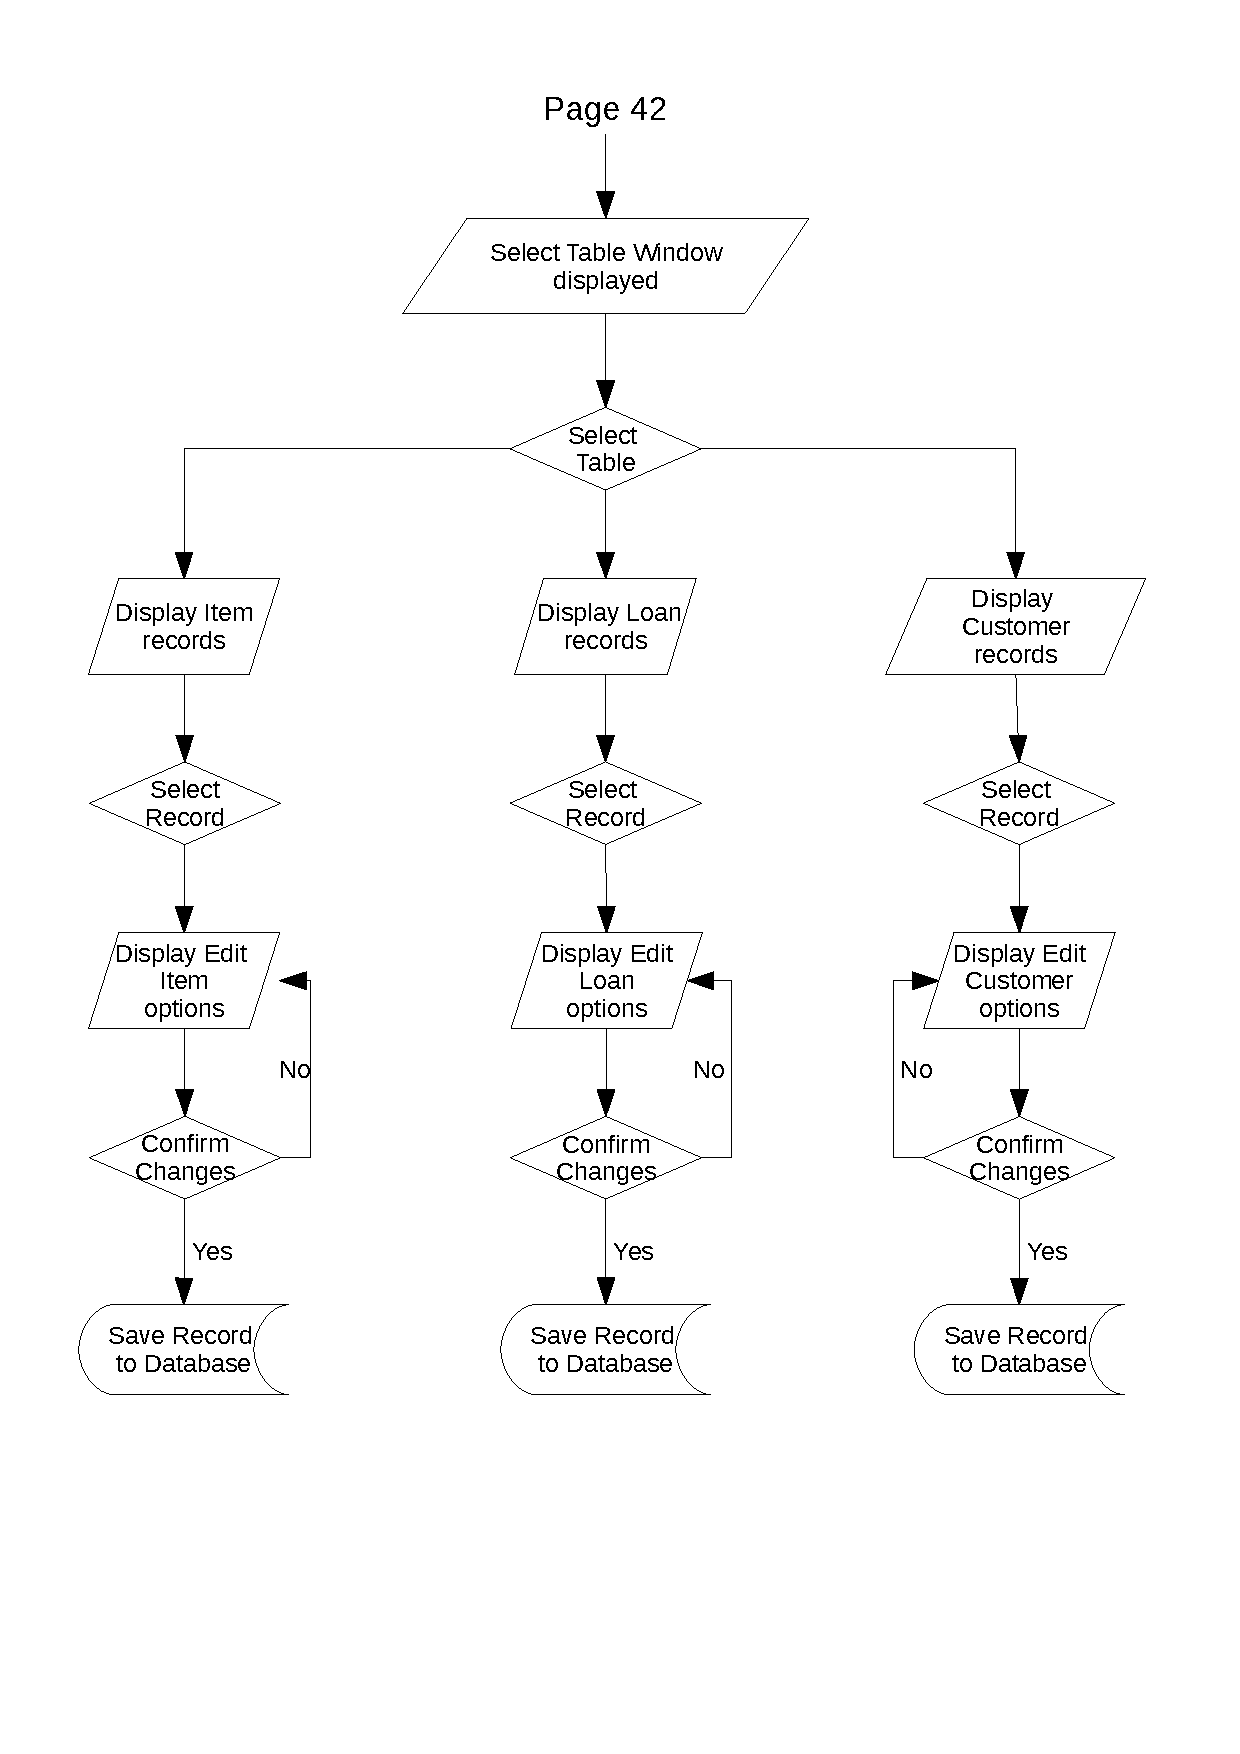
\includegraphics[width=355px]{./Design/system_flowcharts/PDFs/edit_records_flowchart.pdf}
    \end{center}
    \caption{Edit Records Flowchart.} \label{fig:print_function_result}
\end{figure}

\begin{figure}[H]
    \begin{center}
        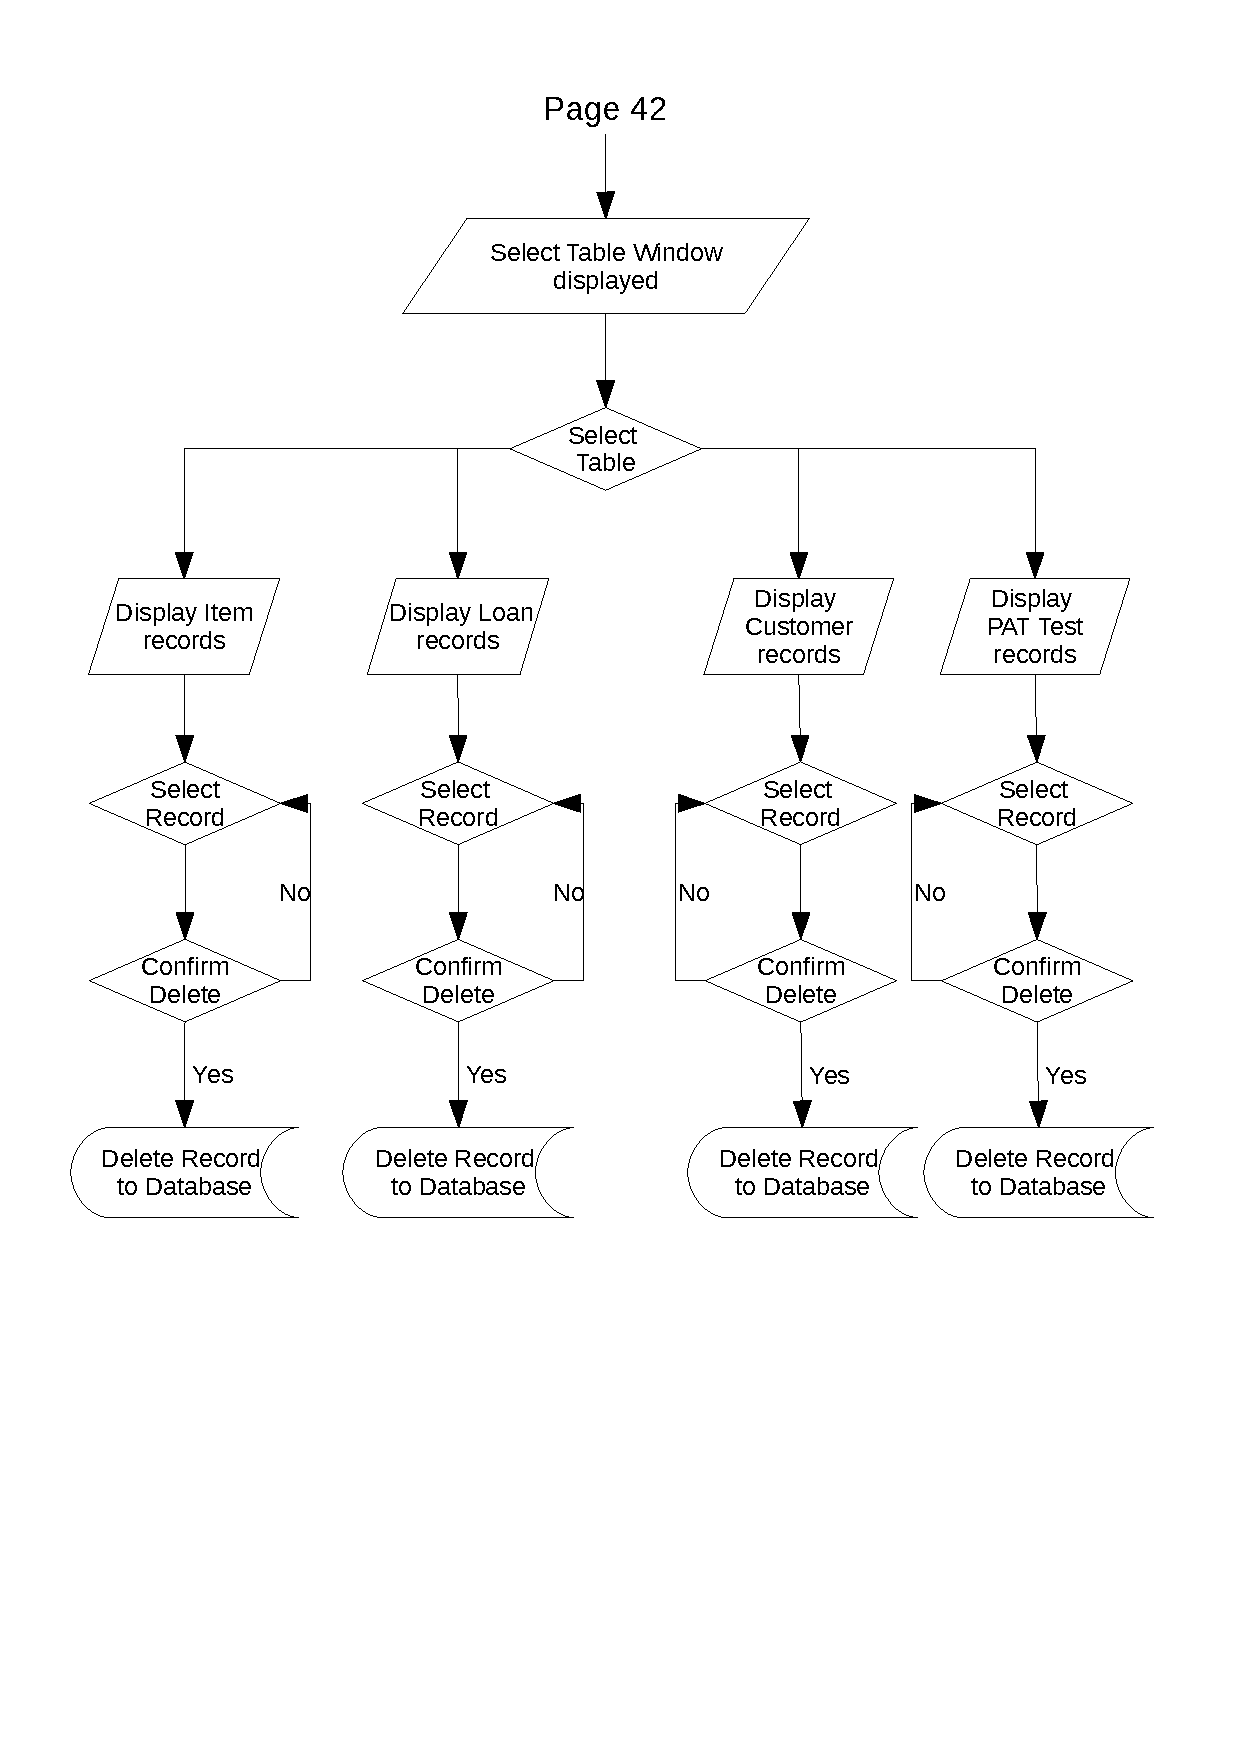
\includegraphics[width=355px]{./Design/system_flowcharts/PDFs/delete_records_flowchart.pdf}
    \end{center}
    \caption{Delete Records Flowchart.} \label{fig:print_function_result}
\end{figure}





\begin{landscape}

\section{User Interface Designs}

\begin{figure}[H]
    \begin{center}
        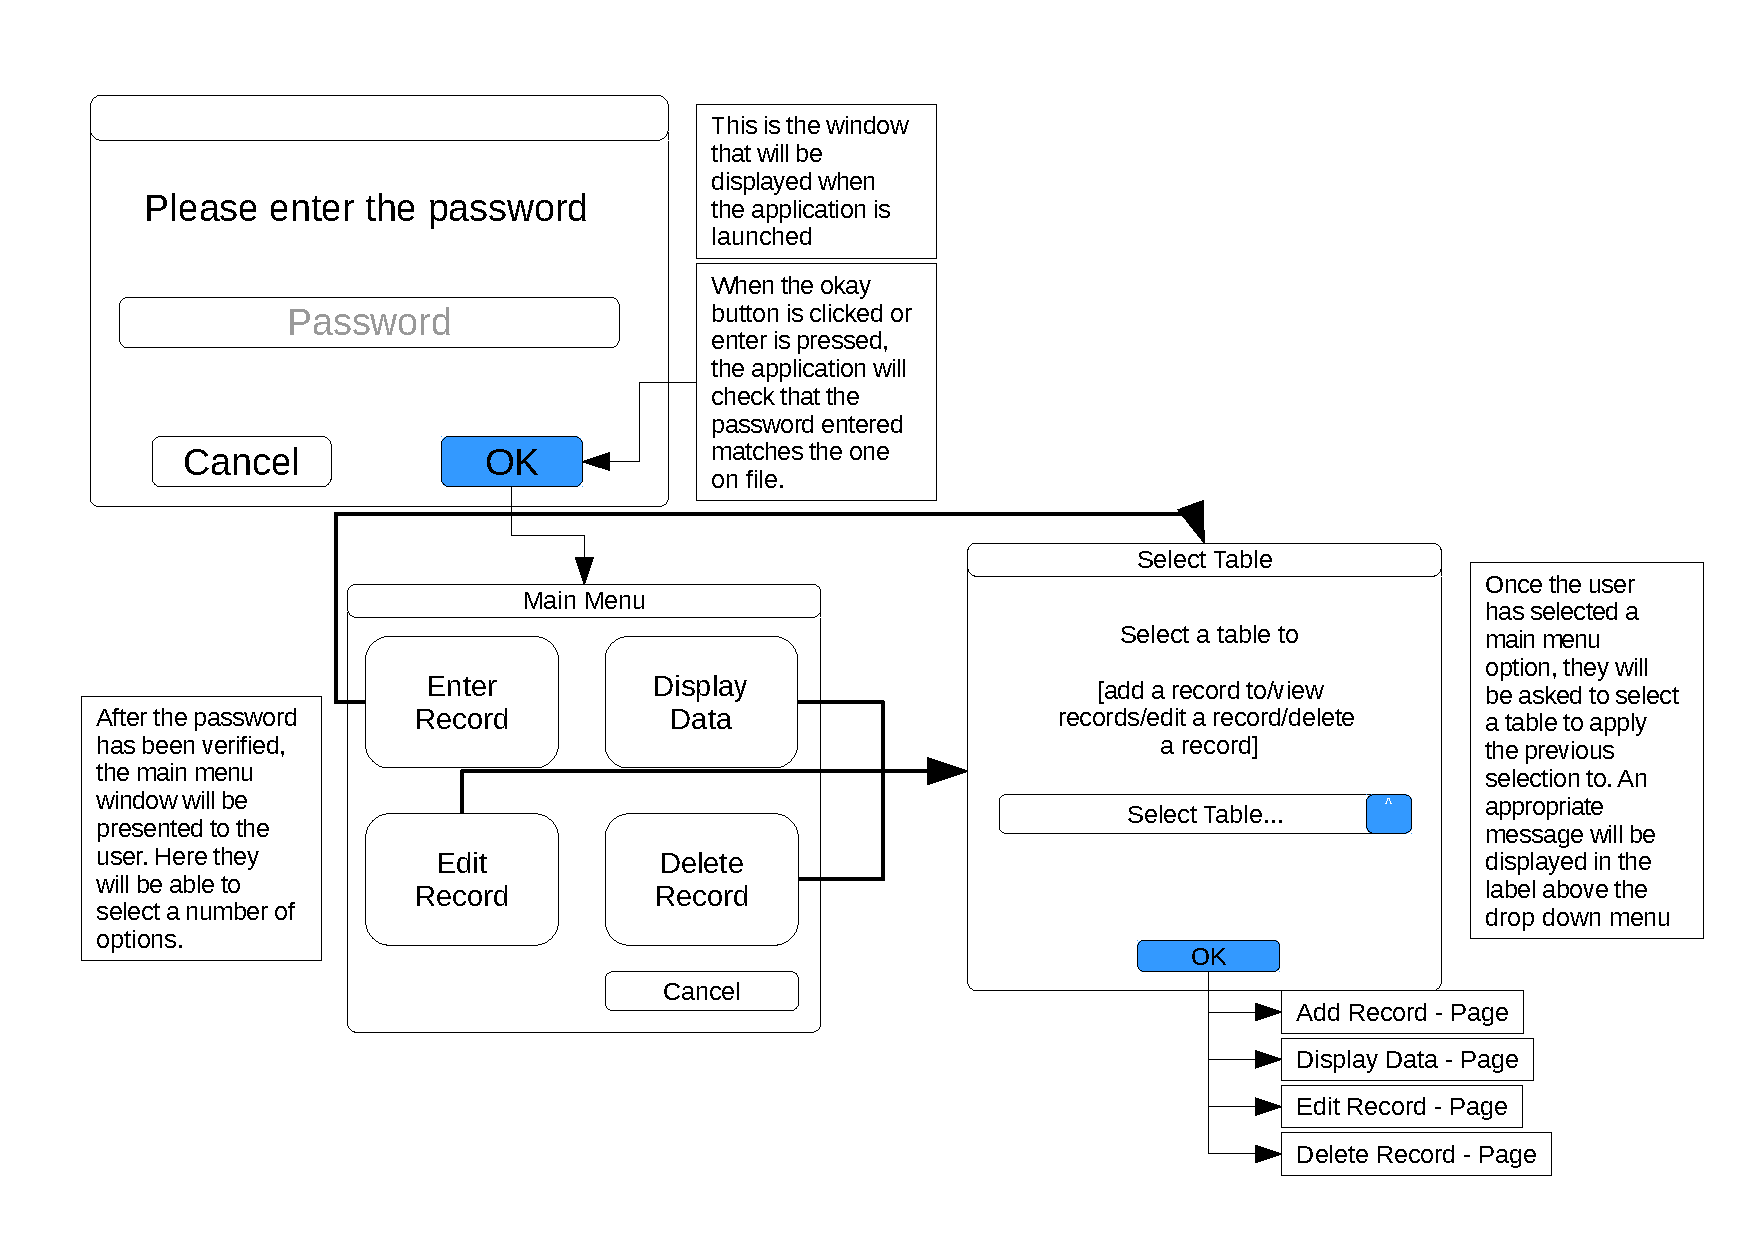
\includegraphics[width=420px]{./Design/user_interface/login_interface.pdf}
    \end{center}
    \caption{Login and Main Menu windows.} \label{fig:print_function_result}
\end{figure}

\begin{center}
    Clicking the "Logout" button will return you to the login screen.
\end{center}

\newpage

\begin{figure}[H]
    \begin{center}
        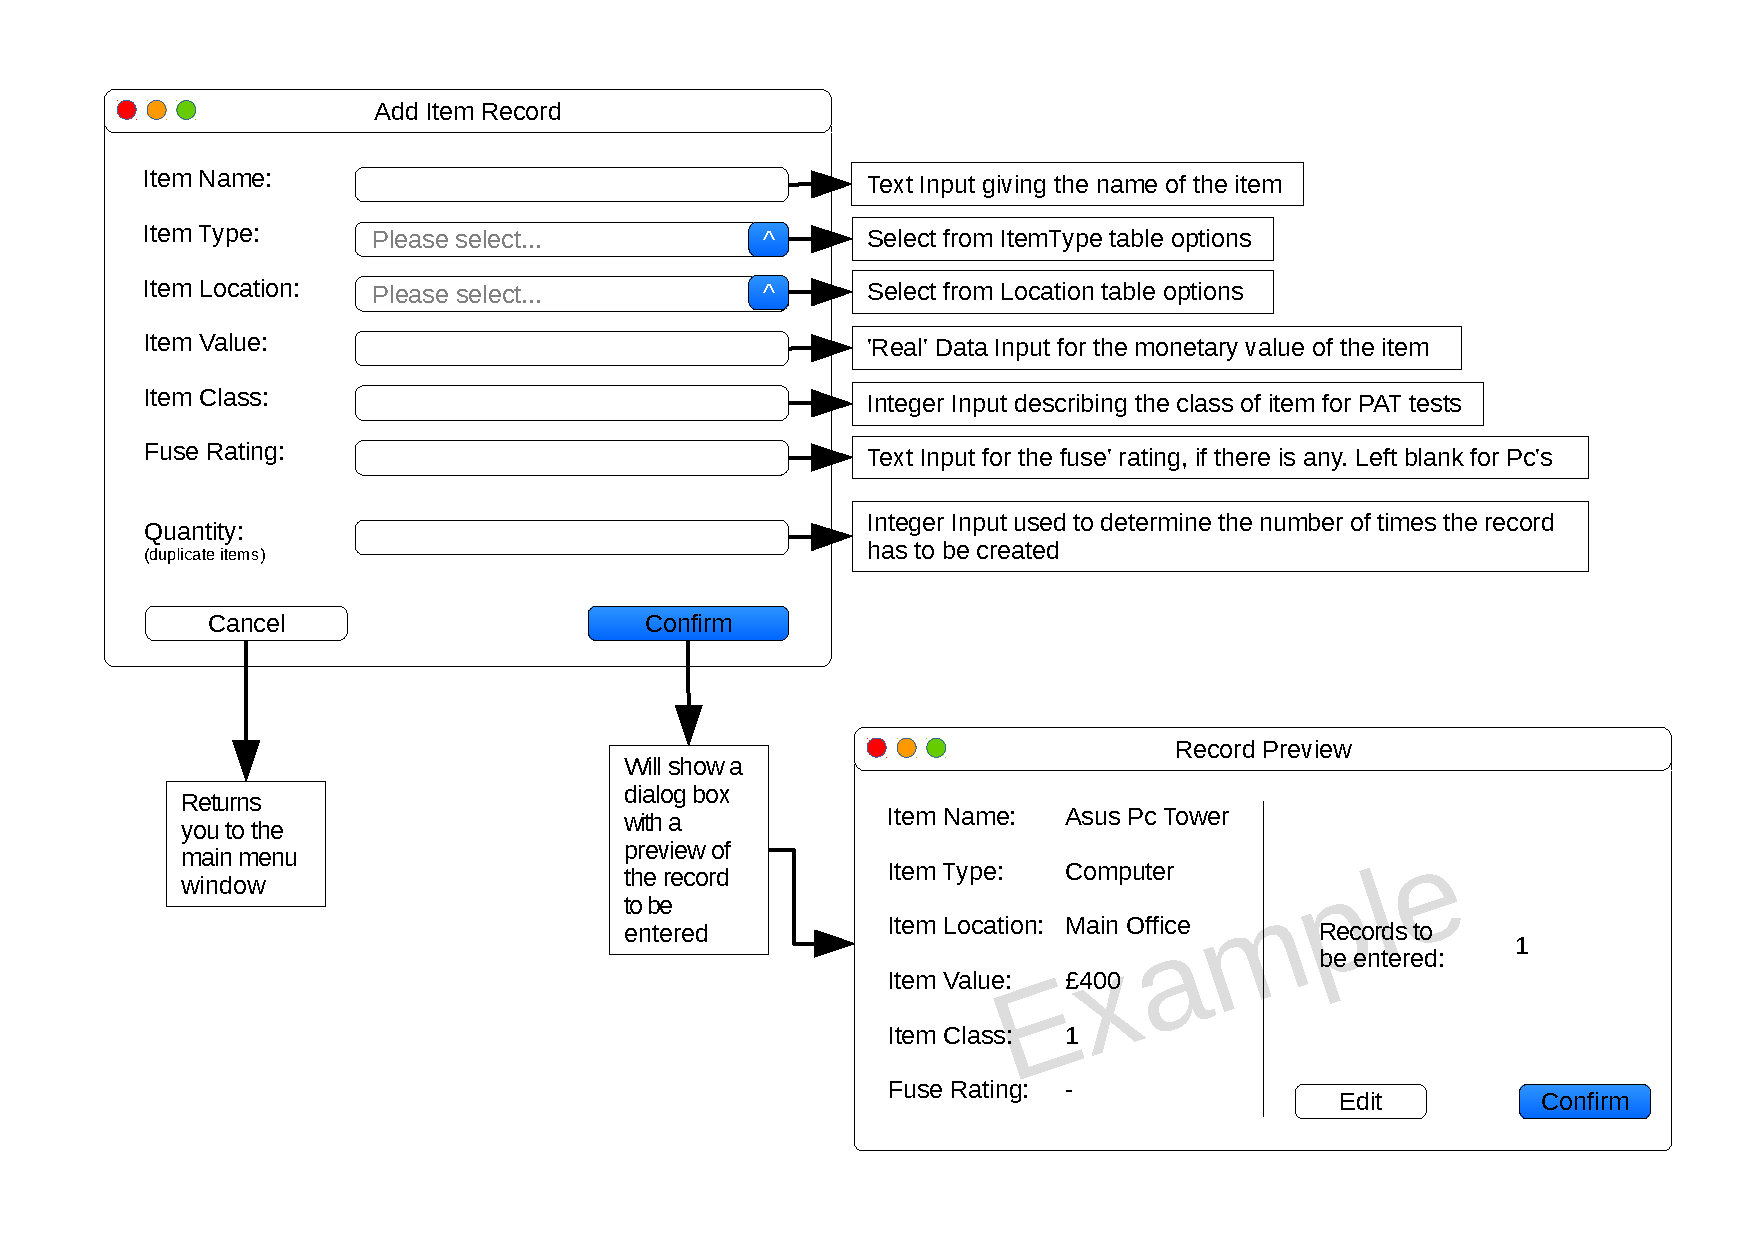
\includegraphics[width=500px]{./Design/user_interface/Add_item_record_interface.pdf}
    \end{center}
    \caption{Login and Main Menu windows.} \label{fig:print_function_result}
\end{figure}

\newpage

\begin{figure}[H]
    \begin{center}
        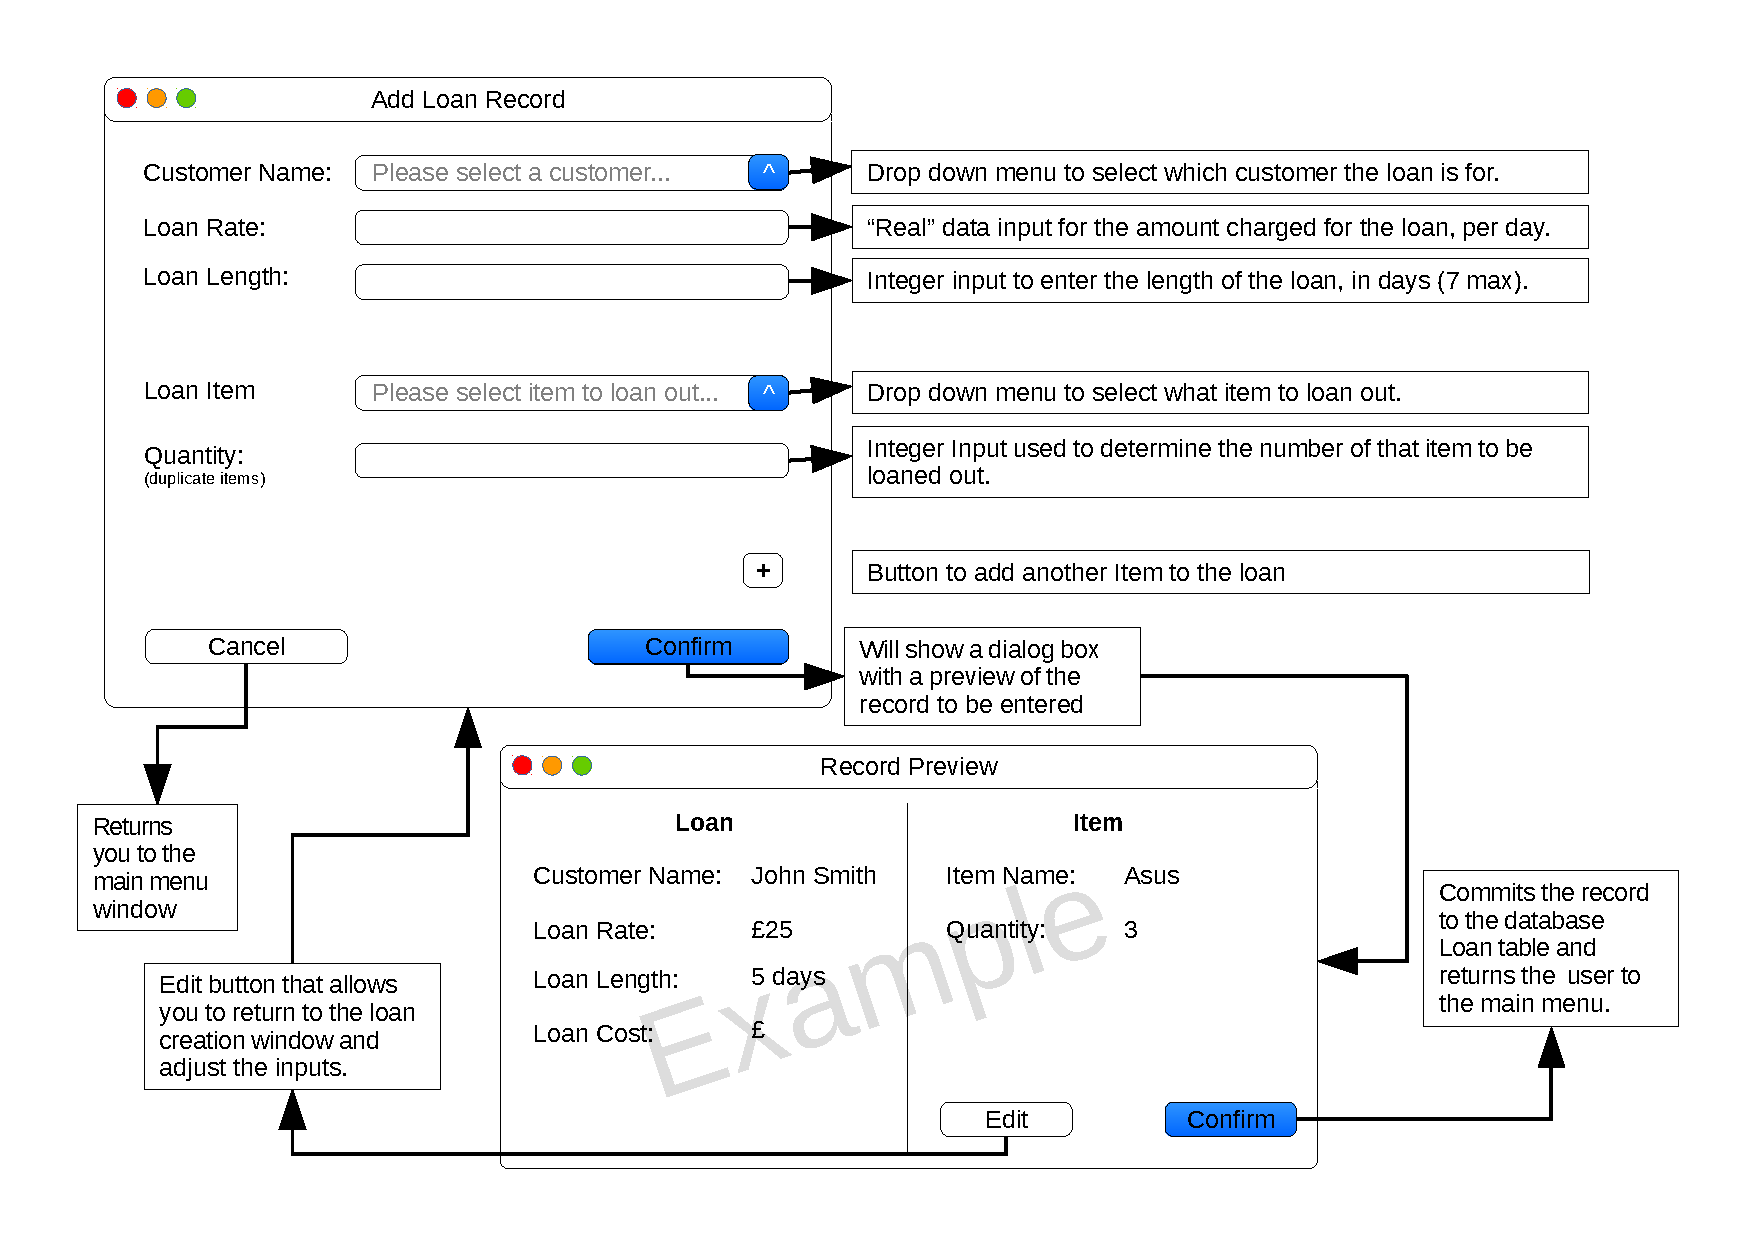
\includegraphics[width=500px]{./Design/user_interface/Add_loan_record_interface.pdf}
    \end{center}
    \caption{Login and Main Menu windows.} \label{fig:print_function_result}
\end{figure}

\newpage

\begin{figure}[H]
    \begin{center}
        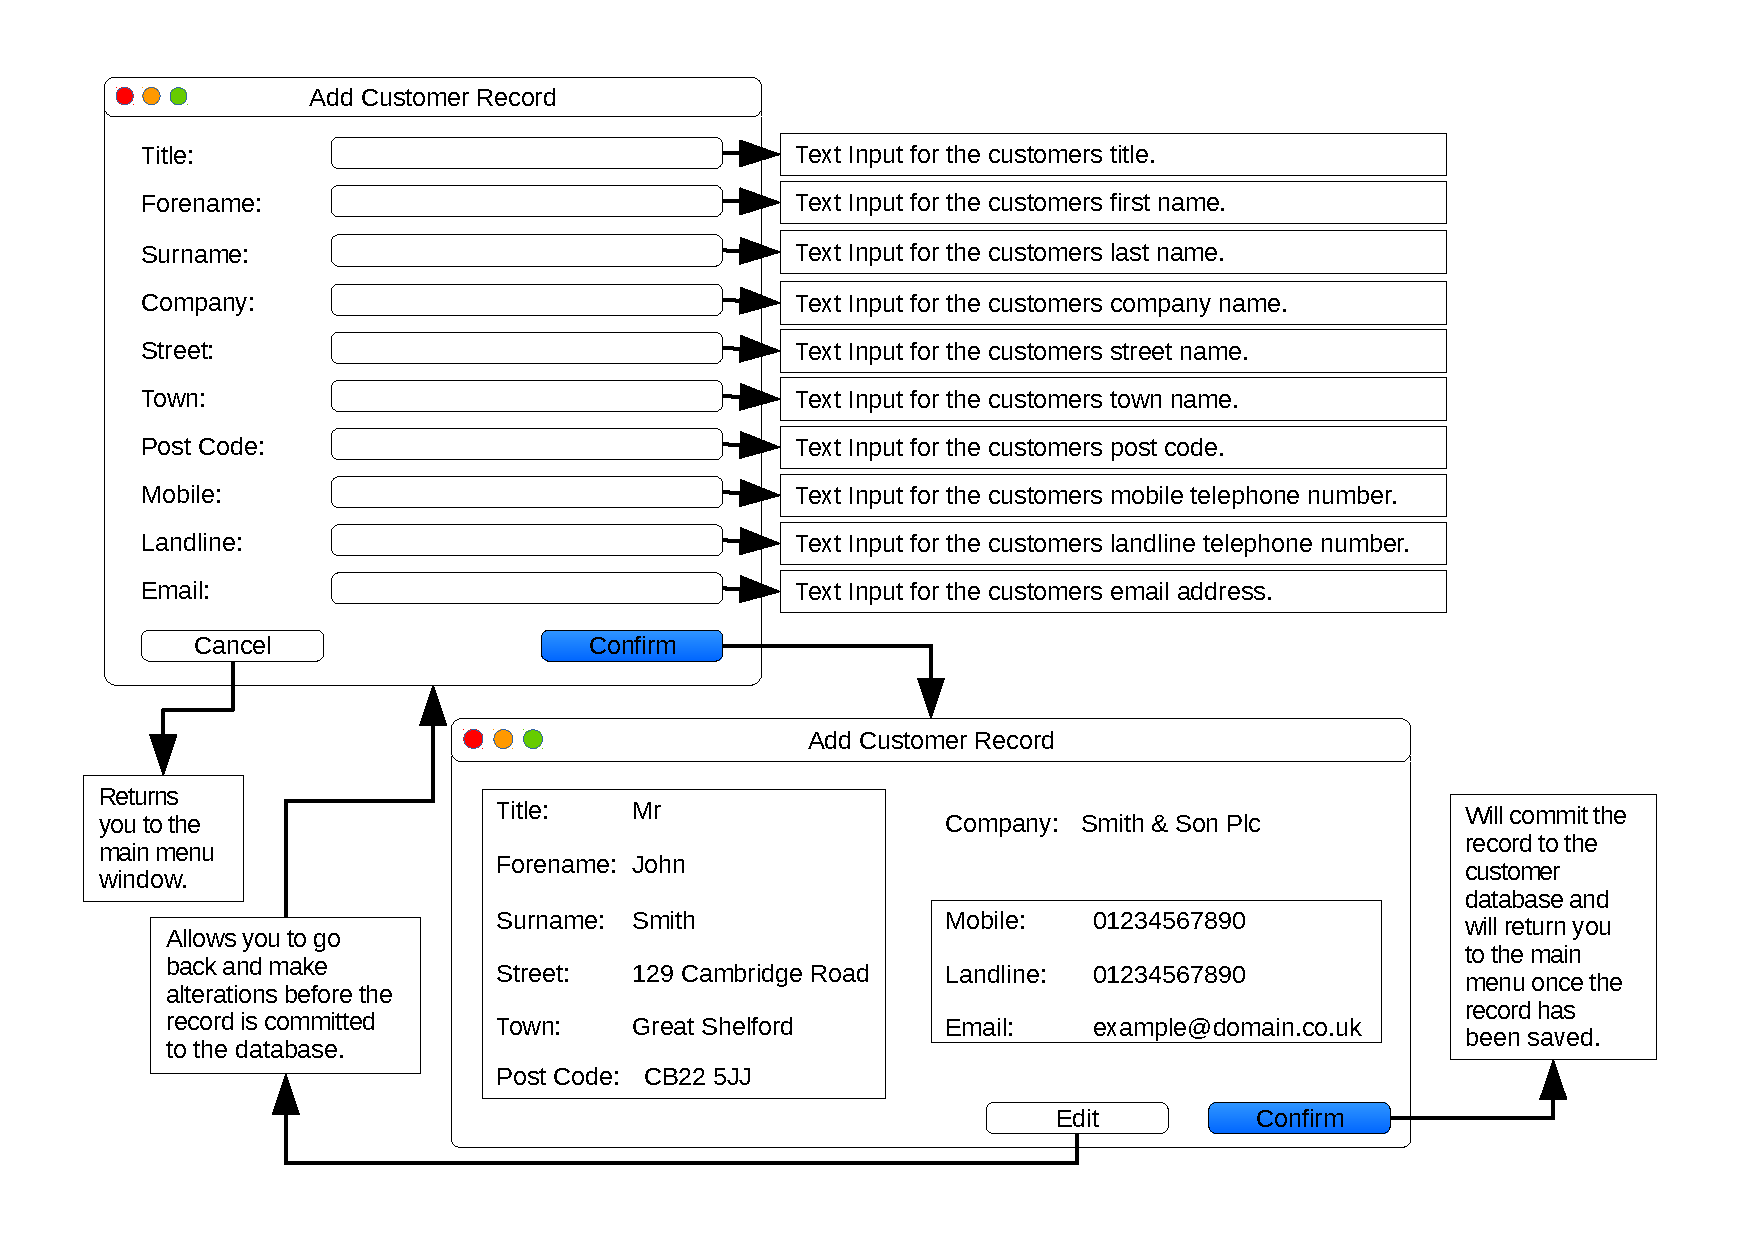
\includegraphics[width=500px]{./Design/user_interface/Add_customer_record_interface.pdf}
    \end{center}
    \caption{Login and Main Menu windows.} \label{fig:print_function_result}
\end{figure}

\newpage

\begin{figure}[H]
    \begin{center}
        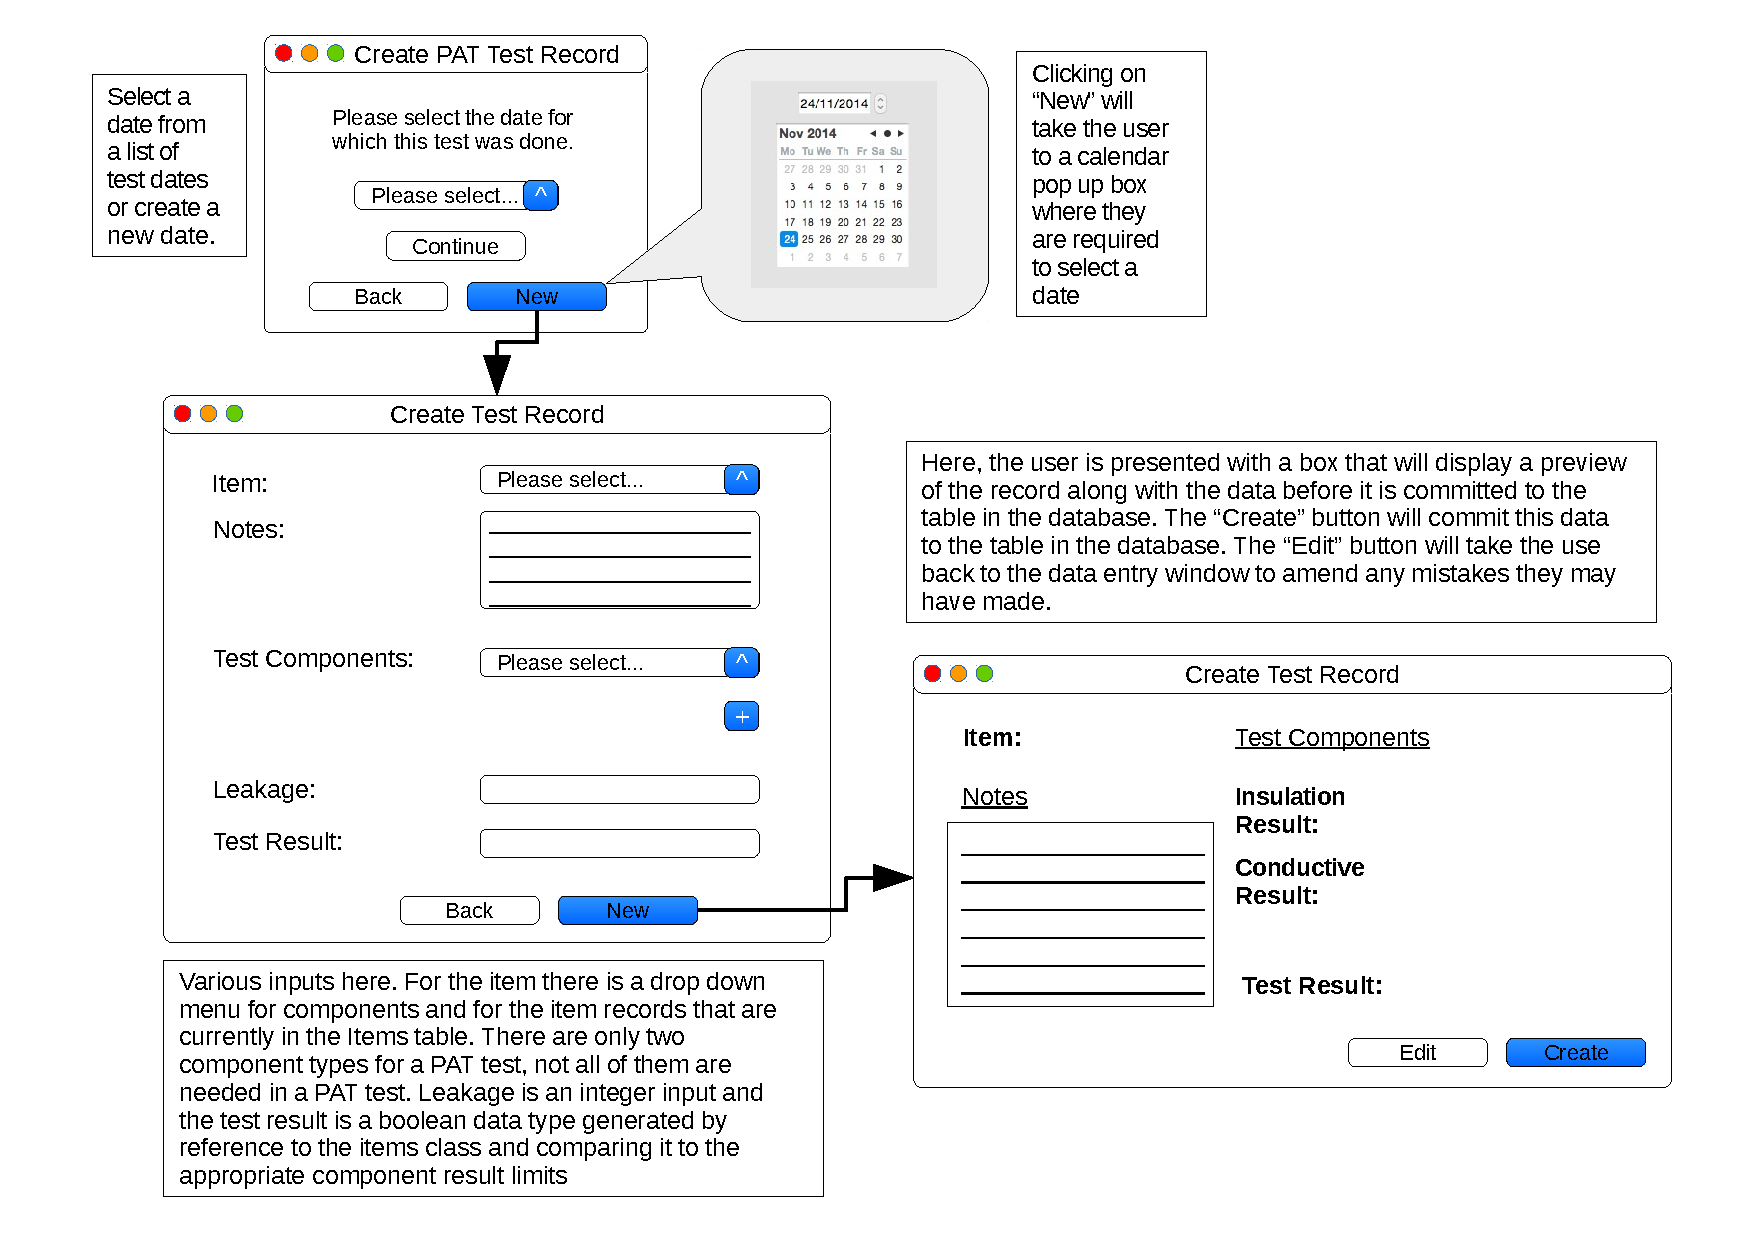
\includegraphics[width=500px]{./Design/user_interface/Add_pat_test_record_interface.pdf}
    \end{center}
    \caption{Login and Main Menu windows.} \label{fig:print_function_result}
\end{figure}

\newpage

\begin{figure}[H]
    \begin{center}
        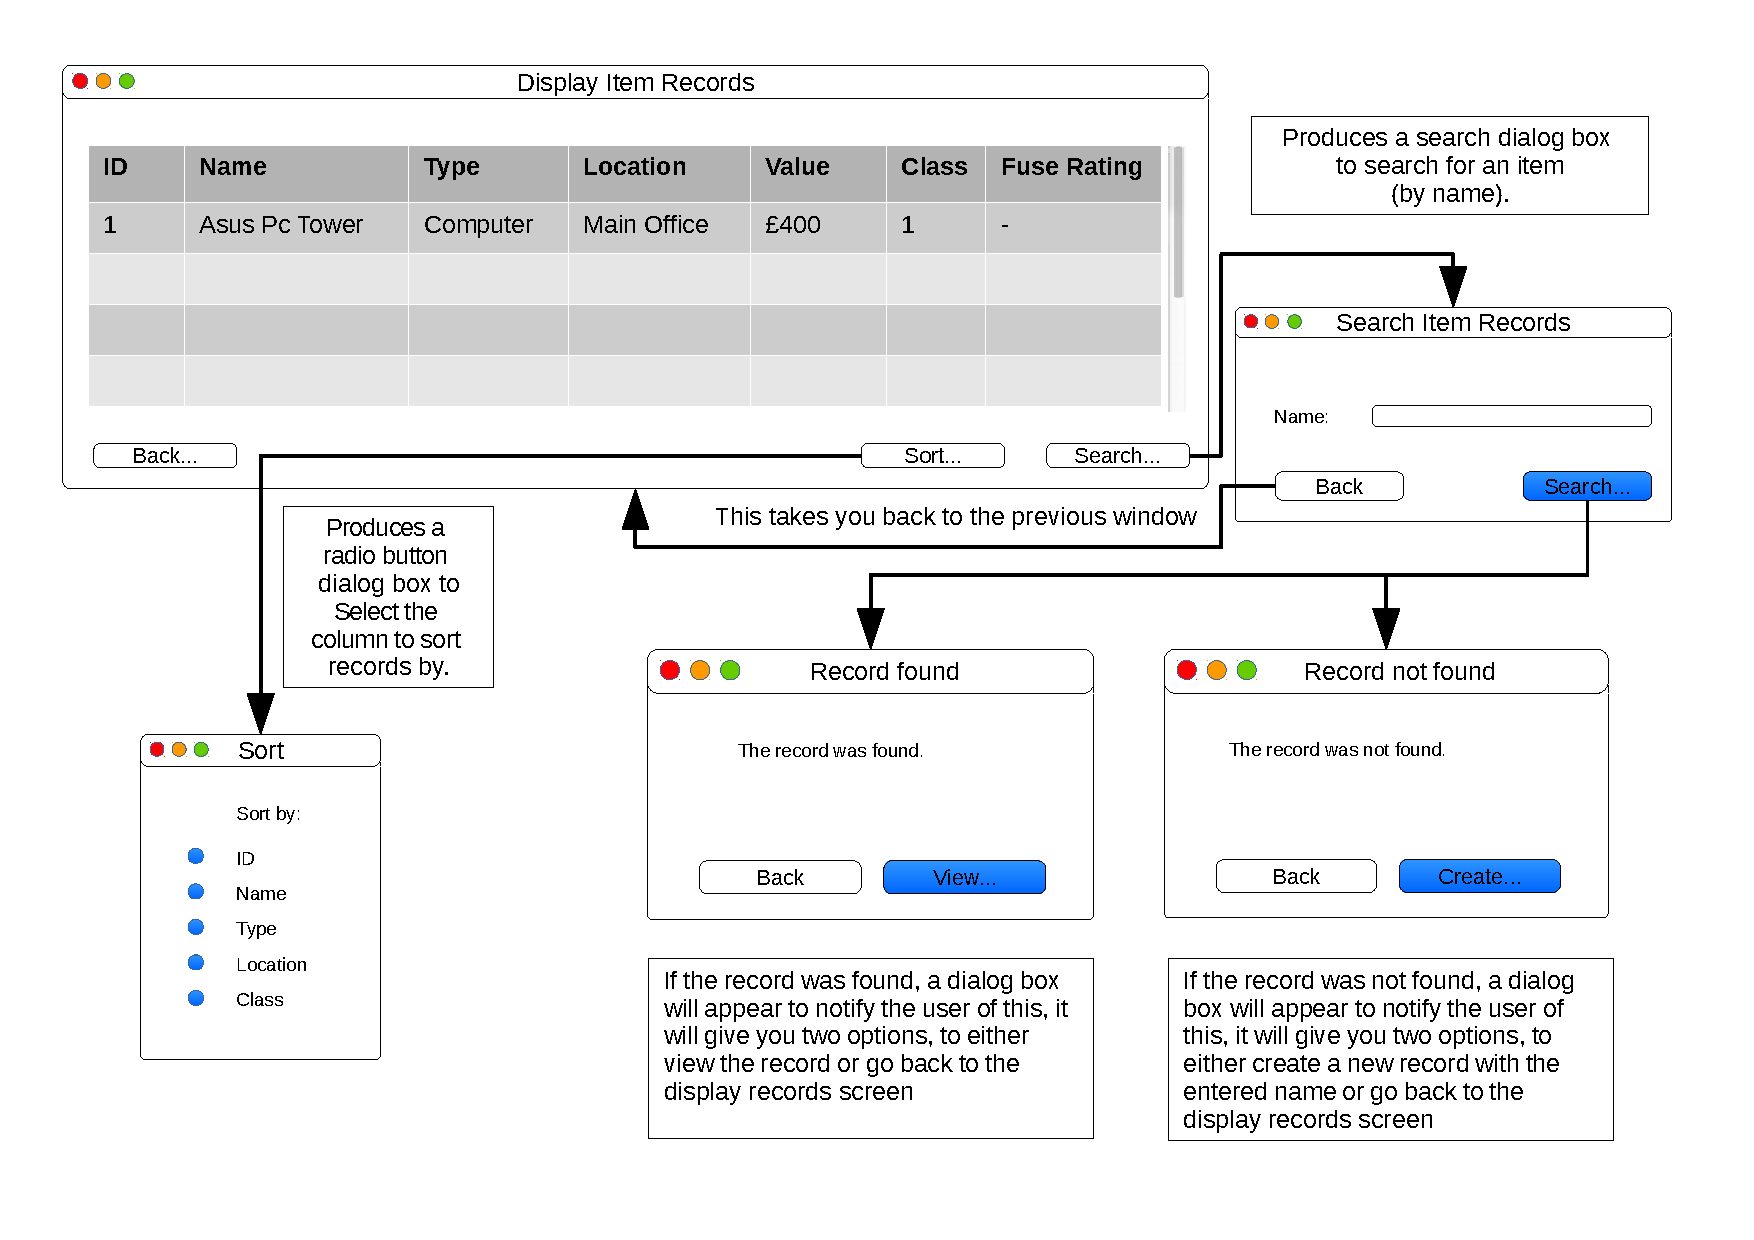
\includegraphics[width=500px]{./Design/user_interface/Display_item_records_interface.pdf}
    \end{center}
    \caption{Login and Main Menu windows.} \label{fig:print_function_result}
\end{figure}

\end{landscape}

\section{Hardware Specification}

The hardware I am going to use are for a custom built Early 2008 Mac Pro. The specifications are as follows:
\begin{itemize}
    \item 2x 2.8 GHz Quad-Core Intel\textregistered Xeon\texttrademark Processor
    \item ATI Radeon HD 2600 XT 256MB Graphics Card
    \item 661-4449 Apple Mac Pro A1186 Motherboard
    \item 16.00GB DDR3 RAM
    \item 1TB SATA Disk-Drive
    \item 6TB RAID Storage
    \item Apple SuperDrive \\
\end{itemize}

I have chosen to build my system for this specification as this is the computer my client is going to run the application on, it is also a low cost choice of system spec to run on as the hardware has already been bought and is therefore ready and available to use.

\section{Program Structure}

\begin{landscape}

    \subsection{Top-down design structure charts}

    \begin{figure}[H]
        \begin{center}
        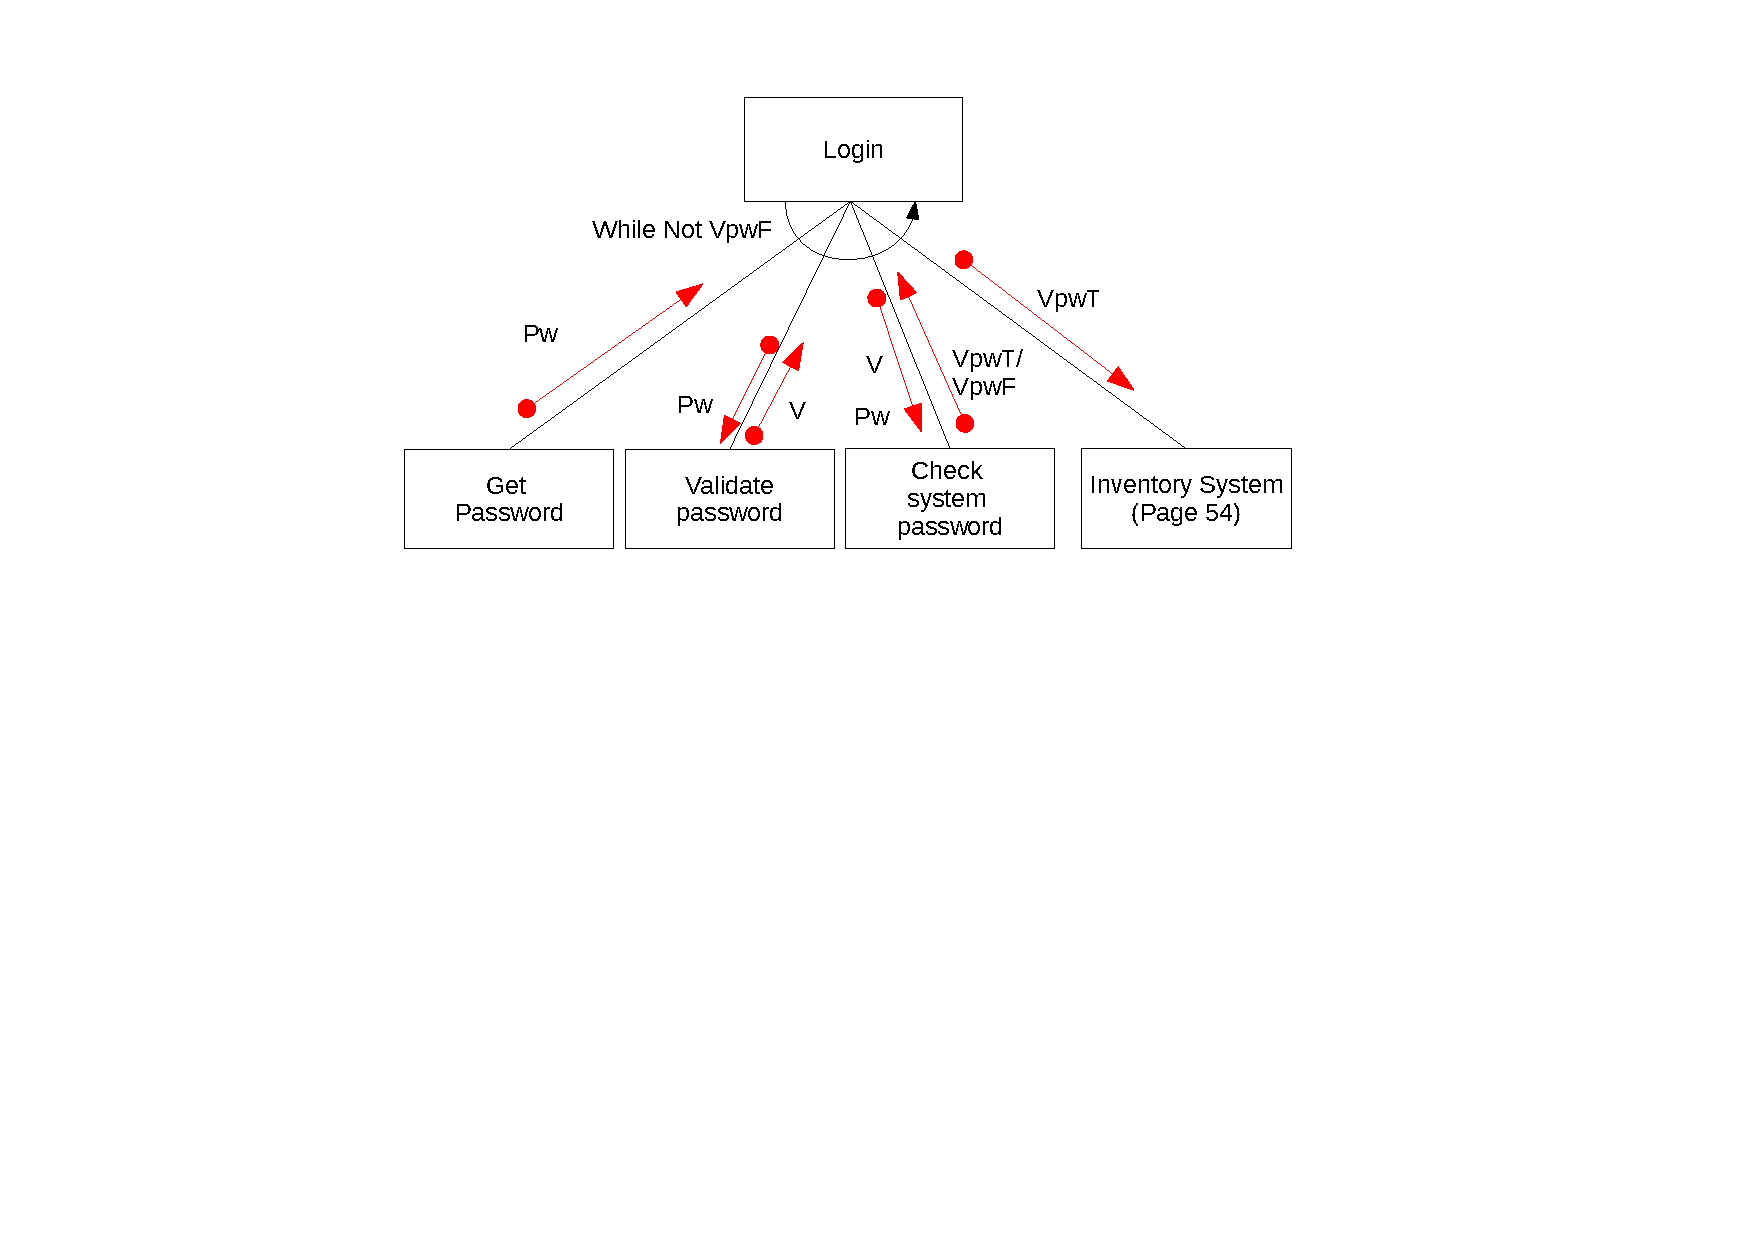
\includegraphics[width=500px]{./Design/top_down_design/Top_down_design.pdf}
        \caption{Object Diagram.} \label{fig:object_diagram}
        \end{center}
    \end{figure}

\end{landscape}


\subsection{Algorithms in pseudo-code for each data transformation process}

\begin{landscape}

    \subsection{Object Diagrams}

    \begin{figure}[H]
        \begin{center}
        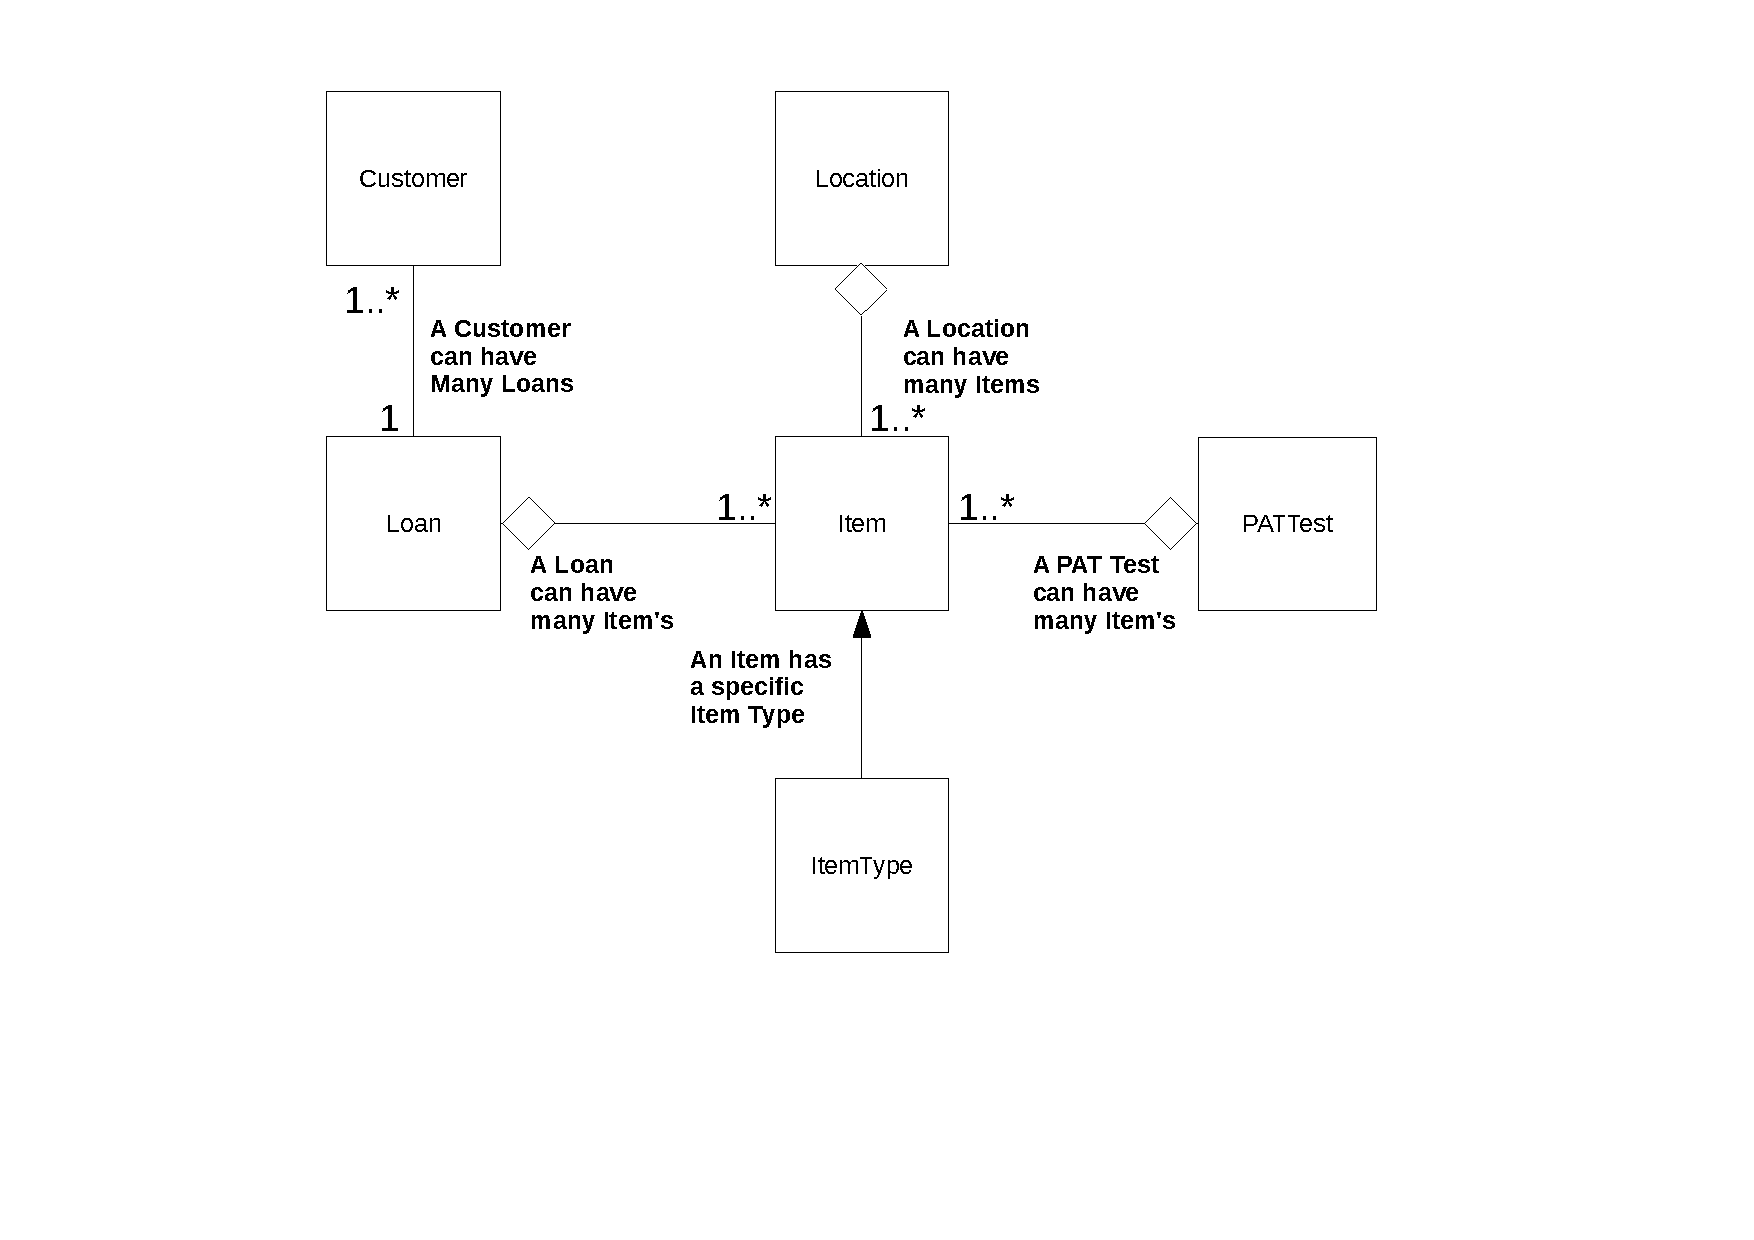
\includegraphics[width=500px]{./Design/Object_Diagrams/Object_diagrams.pdf}
        \caption{Object Diagram.} \label{fig:object_diagram}
        \end{center}
    \end{figure}

\newpage

\subsection{Class Definitions}

    \begin{figure}[H]
        \centerline{\includegraphics[width=50px]{./Design/Class_Definitions/Class_definition_key.pdf}}
        \caption{Class Diagram Key.} \label{fig:relationship_diagram}
    \end{figure}

    \begin{figure}[H]
        \centerline{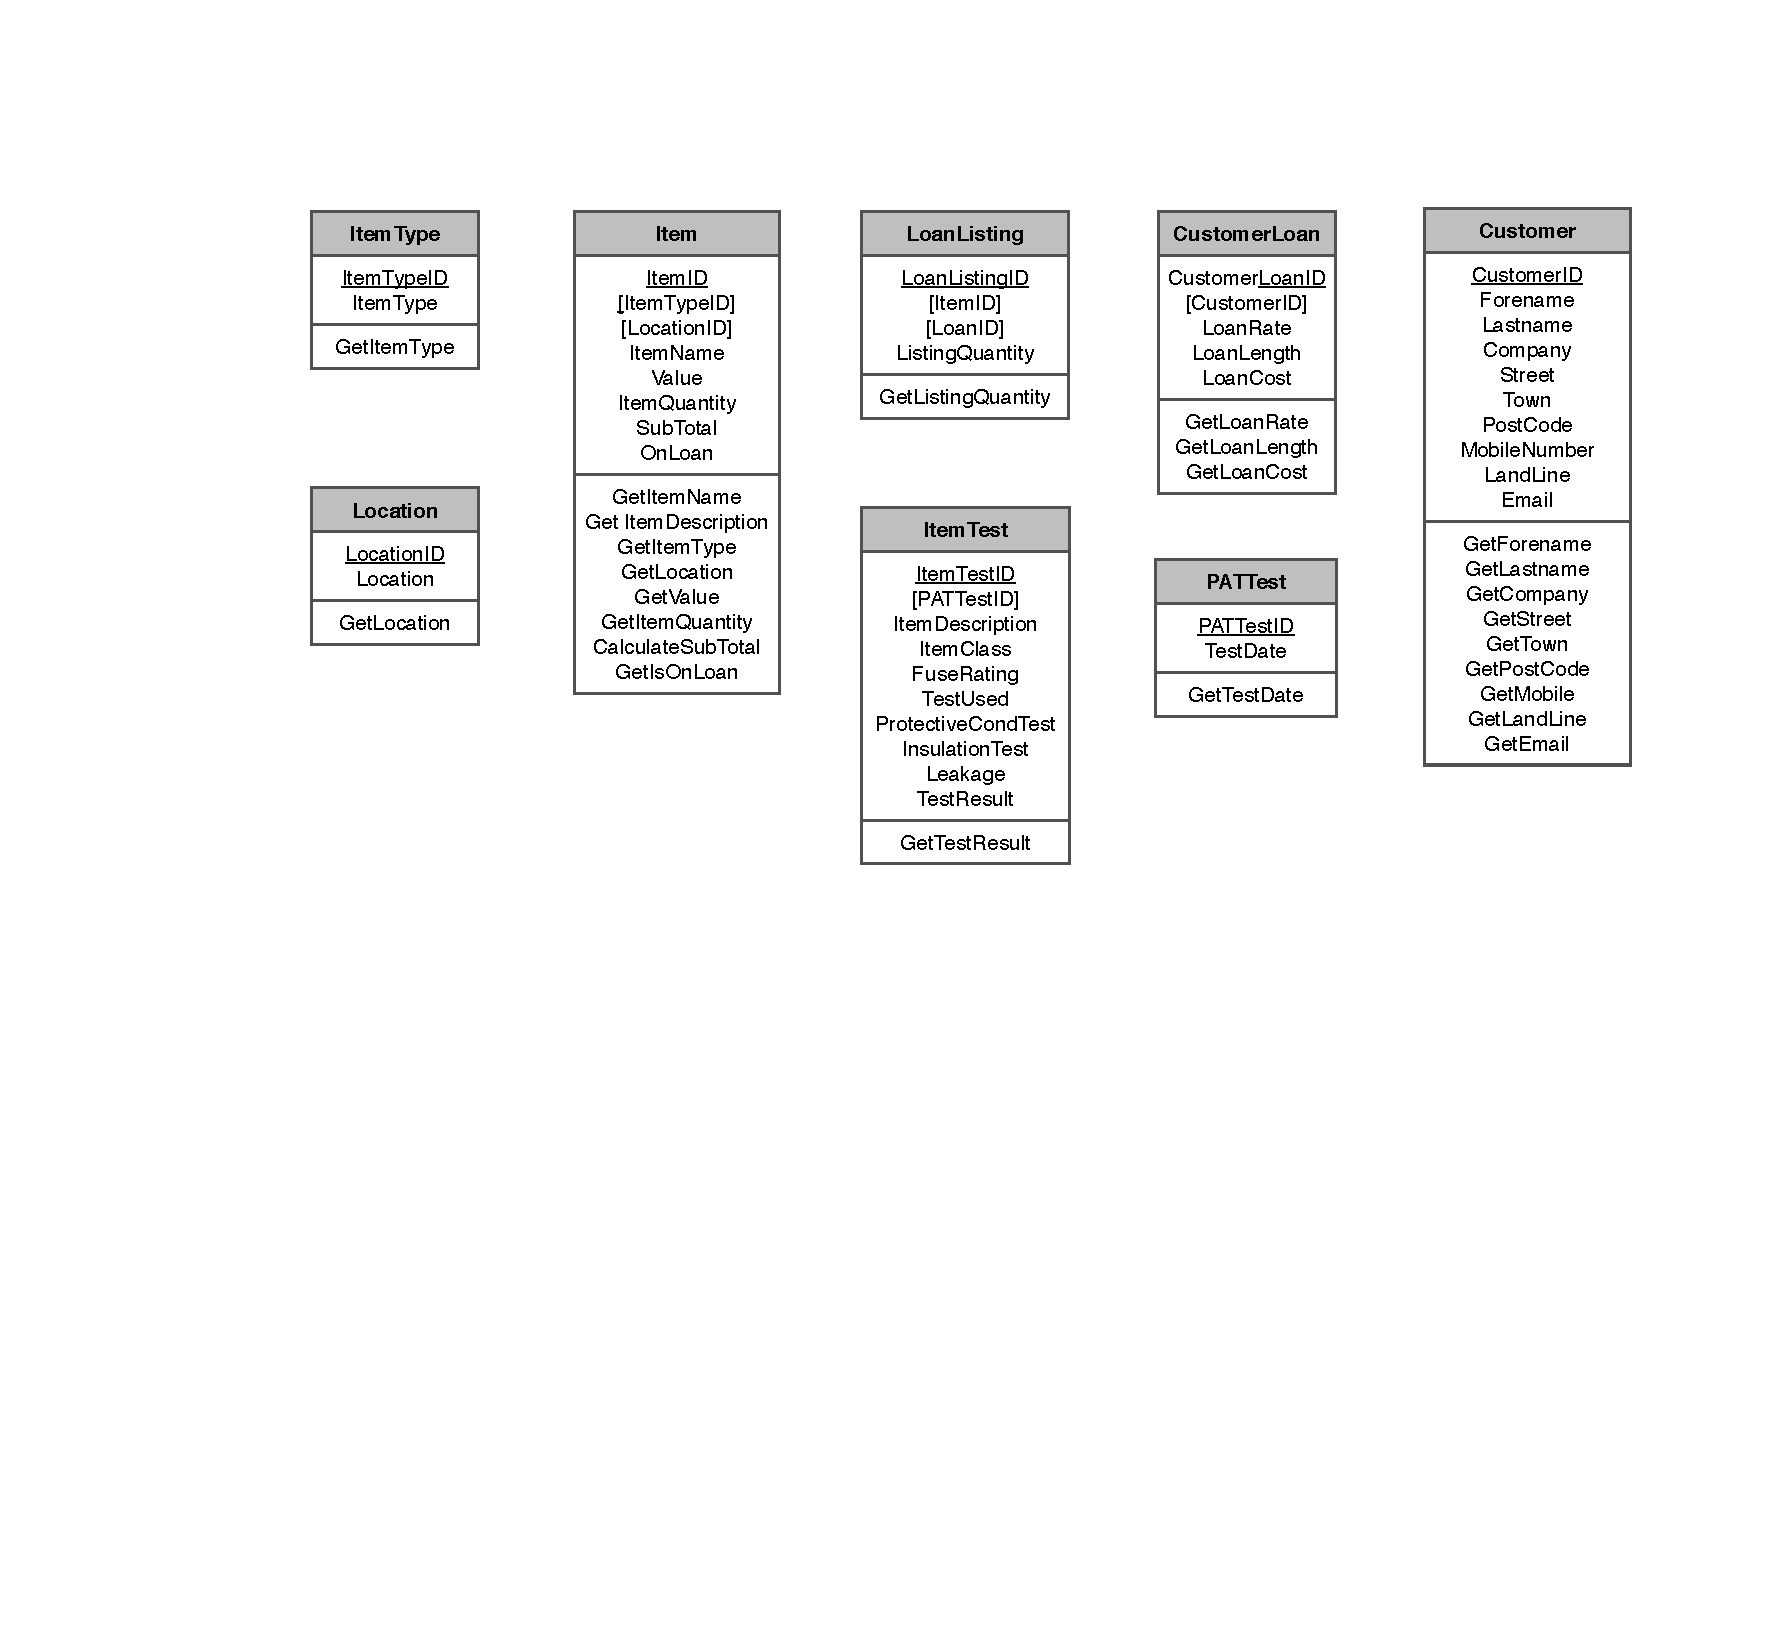
\includegraphics[width=450px]{./Design/Class_Definitions/Class_definitions.pdf}}
        \caption{Class Diagrams.} \label{fig:relationship_diagram}
    \end{figure}


\end{landscape}

\newpage

\section{Prototyping}

\section{Definition of Data Requirements}

\subsection{Identification of all data input items}

\subsection{Identification of all data output items}

\subsection{Explanation of how data output items are generated}

\subsection{Data Dictionary}

\subsection{Identification of appropriate storage media}

\section{Database Design}

\newpage

\begin{landscape}

\subsection{ER Diagrams}

\begin{figure}[H]
    \centerline{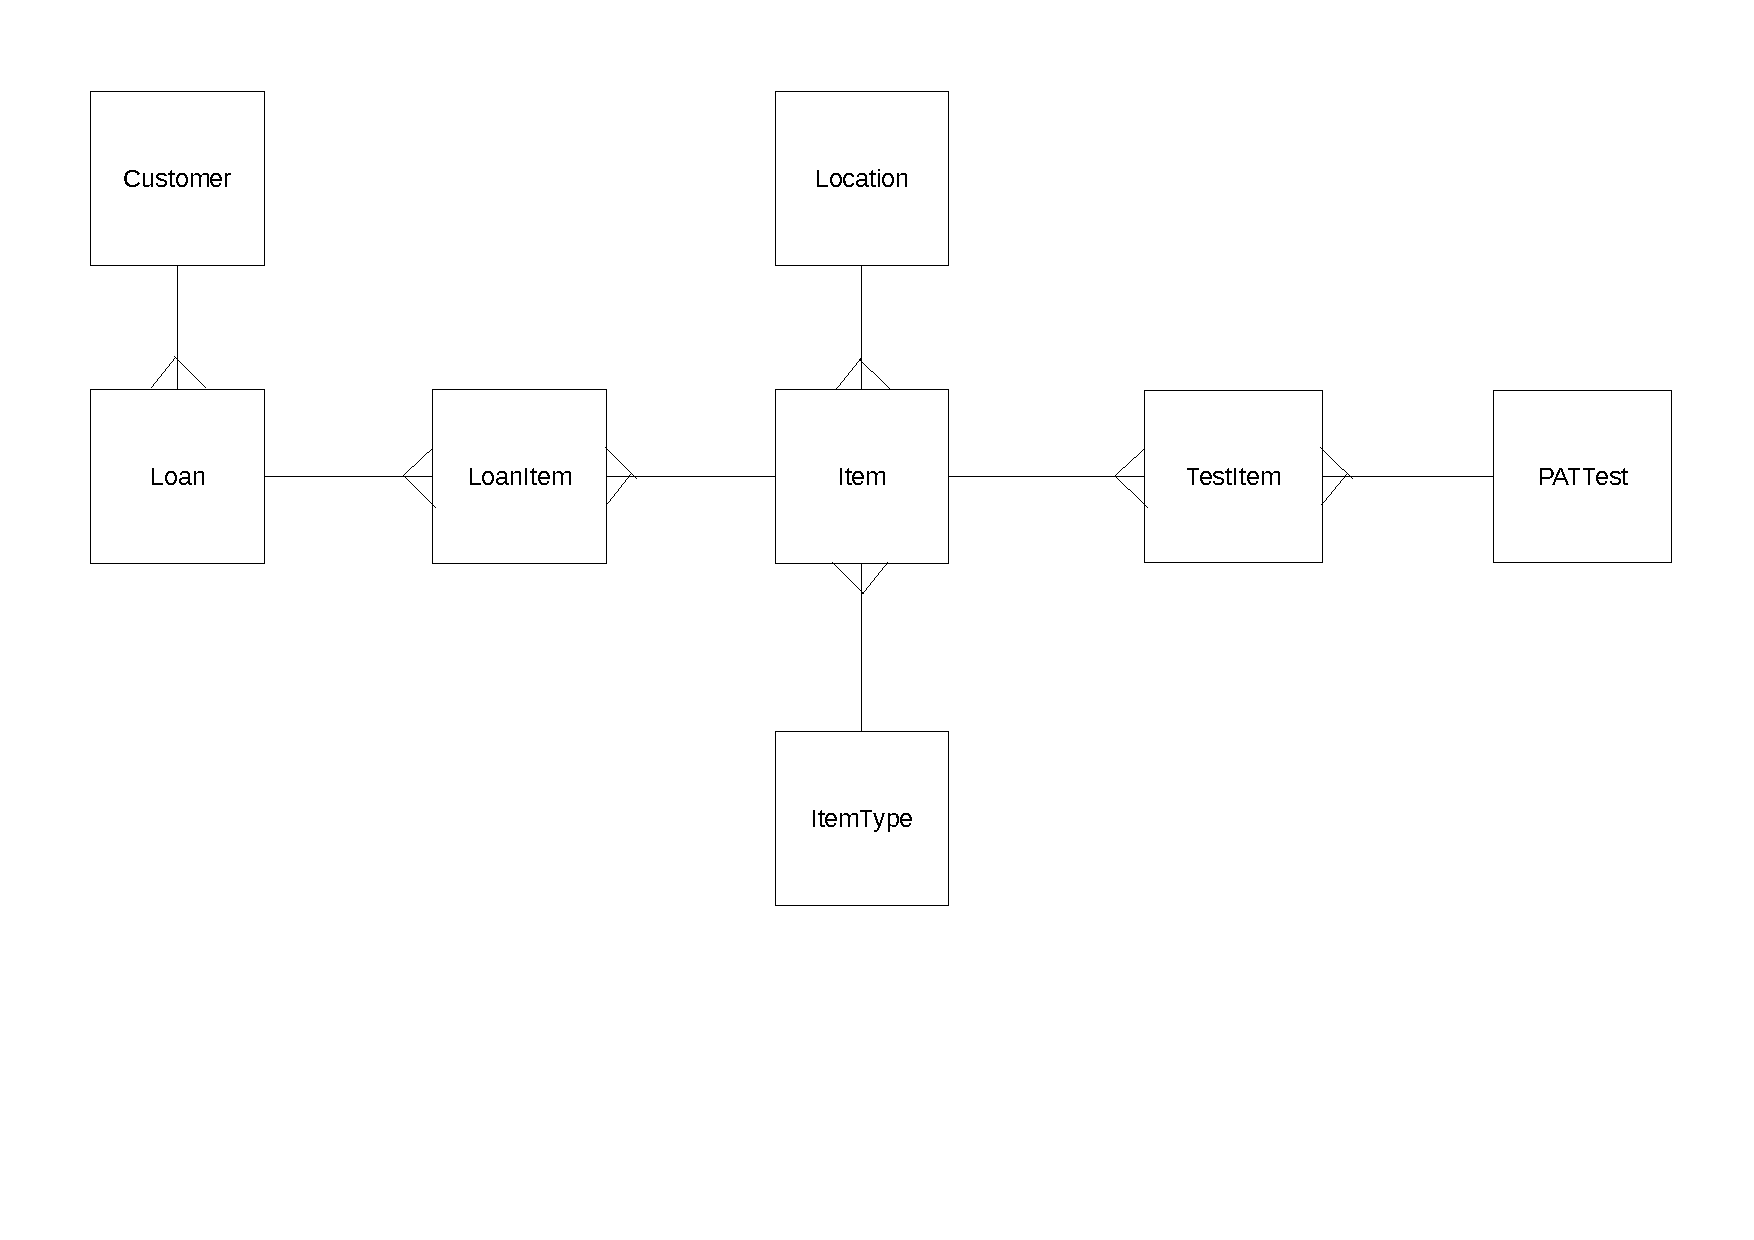
\includegraphics[width=600px]{./Design/ER_Diagrams/ER_Diagram.pdf}}
    \caption{ER Diagrams.} \label{fig:ER Diagrams}
\end{figure}

\end{landscape}

\subsection{Entity Descriptions}

\noindent \textbf{Location}(\underline{LocationID}, Location)

\noindent \textbf{ItemType}(\underline{ItemTypeID}, ItemType)

\noindent \textbf{Item}(\underline{ItemID}, \emph{LocationID}, \emph{ItemTypeID}, ItemName, Value, LoanRate, ItemClass, FuseRating, )

\noindent \textbf{Customer}(\underline{CustomerID}, Forename, Surname, Company, Street, Town, PostCode, MobileNumber, Landline, Email)

\noindent \textbf{Loan}(\underline{LoanID}, \emph{CustomerID}, StartDate, LoanLength)

\noindent \textbf{LoanItem}(\underline{LoanItemID}, \emph{LoanID}, \emph{ItemID}, Quantity)

\noindent \textbf{PATtest}(\underline{PATtestID}, TestDate)

\noindent \textbf{ItemTest}(\underline{ItemTestID}, \emph{ItemID}, PATtestNotes, ComponentType, ComponentResult, ComponentNotes, Leakage, TestResult)

\subsection{Normalisation}

\subsubsection{UNF to 3NF}

\begin{center}
    \begin{tabular}{|c|}
        \hline
        \textbf{Un-Normalised Form(UNF)}\\ \hline
        \underline{ItemID}              \\
        ItemName                        \\
        ItemType                        \\
        Location                        \\ 
        Value                           \\ 
        LoanID                          \\ 
        LoanRate                        \\ 
        LoanLength                      \\ 
        CustomerID                      \\ 
        Forename                        \\ 
        Lastname                        \\ 
        Company                         \\ 
        Street                          \\ 
        Town                            \\ 
        PostCode                        \\ 
        MobileNumber                    \\ 
        LandLine                        \\ 
        Email                           \\ 
        PATtestID                       \\
        TestResult                      \\ 
        TestDate                        \\ 
        ItemDescription                 \\ 
        ItemClass                       \\ 
        FuseRating                      \\ 
        PATTestNotes                    \\ 
        ComponentType                   \\
        ComponentResult                 \\
        ComponentNotes                  \\
        Leakage                         \\ \hline
    \end{tabular}
\end{center}

\newpage

\begin{center}
    \begin{tabular}{|c|c|}
        \hline
        \multicolumn{2}{|c|}{\textbf{First-Normalised Form(1NF)}} \\
        \multicolumn{2}{|c|}{ }                                   \\ \hline
        \textbf{Non-Repeating} & \textbf{Repeating}               \\ \hline
        \underline{ItemID}     & \underline{LoanID}               \\ 
        ItemName               & \emph{ItemID}                    \\ 
        Value	              & LoanRate                         \\ 
        ItemClass	          & LoanLength                       \\ 
        FuseRating             & CustomerID                       \\ 
              	              & Forename                         \\ 
              	              & Lastname                         \\ 
                               & Company                          \\ 
                               & Street                           \\ 
                               & Town                             \\ 
                               & PostCode                         \\ 
                               & MobileNumber                     \\ 
                               & Landline                         \\ 
                               & Email                            \\ 
                               & PATtestID                        \\ 
                               & TestDate                         \\ 
                               & PATTestNotes                     \\ 
                               & ComponentType                    \\
                               & ComponentResult                  \\
                               & ComponentNotes                   \\
                               & Leakage                          \\ 
                               & TestResult                       \\ \hline
    \end{tabular}
\end{center}

\newpage

\begin{center}
    \begin{tabular}{|c|c|}
        \hline
        \multicolumn{2}{|c|}{\textbf{Second-Normalised Form(2NF)}} \\
        \multicolumn{2}{|c|}{ }                                    \\ \hline
        \textbf{Non-Repeating} & \textbf{Repeating}                \\ \hline
        \underline{ItemID}     & \underline{LoanID}                \\ 
        ItemName               & \emph{ItemID}                     \\ 
        Value	              & LoanRate                          \\ 
        ItemClass	          & LoanLength                        \\ 
        FuseRating             & 					                \\
                               &\underline{CustomerID}             \\ 
                               & Forename                          \\ 
              	              & Lastname                          \\ 
                               & Company                           \\ 
                               & Street                            \\ 
                               & Town                              \\ 
                               & PostCode                          \\ 
                               & MobileNumber                      \\ 
                               & Landline                          \\ 
                               & Email                             \\ 
                               & PATtestID                         \\ 
                               & TestDate                          \\ 
                               & PATTestNotes                      \\ 
                               & ComponentType                     \\
                               & ComponentResult                   \\
                               & ComponentNotes                    \\
                               & Leakage                           \\ 
                               & TestResult                        \\ 
                               & Location                          \\
                               & ItemType                          \\ \hline
    \end{tabular}
\end{center}

\begin{center}
    \begin{tabular}{|c|c|}
        \hline
        \multicolumn{2}{|c|}{\textbf{Third-Normalised Form(3NF)}}  \\
        \multicolumn{2}{|c|}{ }                                    \\ \hline
        \textbf{Non-Repeating}     & \textbf{Repeating}            \\ \hline
        \underline{ItemID}         & \underline{LoanID}            \\
        \emph{LocationID}          & \emph{CustomerID}             \\
        \emph{ItemTypeID}          & LoanLength                    \\
        ItemName                   & \\
        Value	                  &                               \\
        ItemClass                  & \underline{LoanItemID}        \\
        FuseRating                 & \emph{LoanID}                 \\
                                   & \emph{ItemID}                 \\
                                   & Quantity                      \\
                                   &                               \\ 
                                   &\underline{CustomerID}         \\
                                   & Forename                      \\
                                   & Lastname                      \\ 
                                   & Company                       \\ 
                                   & Street                        \\ 
                                   & Town                          \\ 
                                   & PostCode                      \\ 
                                   & MobileNumber                  \\ 
                                   & Landline                      \\ 
                                   & Email                         \\ 
                                   &				                \\
                                   & \underline{PATtestID}         \\
                                   & TestDate                      \\   
                                   &				                \\
                                   & \underline{TestID}            \\
                                   & \emph{PATtestID}              \\
                                   & \emph{ItemID}	                \\
                                   & PATTestNotes                  \\
                                   & ComponentType                 \\
                                   & ComponentResult               \\
                                   & ComponentNotes                \\
                                   & Leakage                       \\ 
                                   & TestResult                    \\ 
                                   &                               \\
                                   & \underline{LocationID}        \\
                                   & Location                      \\
                                   &                               \\
                                   & \underline{ItemTypeID}        \\
                                   & ItemType                      \\ \hline                                
    \end{tabular}
\end{center}

\section{Security and Integrity of the System and Data}

\subsection{Security and Integrity of Data}

\subsection{System Security}

\section{Validation}

\section{Testing}

\begin{landscape}
\subsection{Outline Plan}

\begin{center}
    \begin{tabular}{|p{2cm}|p{5cm}|p{5cm}|p{4cm}|}
        \hline
        \textbf{Test Series} & \textbf{Purpose of Test Series} & \textbf{Testing Strategy} & \textbf{Strategy Rationale}\\ \hline
        Example & Example & Example & Example \\ \hline
    \end{tabular}
\end{center}

\subsection{Detailed Plan}

\begin{center}
    \begin{longtable}{|p{1.5cm}|p{2.5cm}|p{2.5cm}|p{2cm}|p{2cm}|p{2cm}|p{2cm}|p{2cm}|}
        \hline
        \textbf{Test Series} & \textbf{Purpose of Test} & \textbf{Test Description} & \textbf{Test Data} & \textbf{Test Data Type (Normal/ Erroneous/ Boundary)} & \textbf{Expected Result} & \textbf{Actual Result} & \textbf{Evidence}\\ \hline
        Example & Example & Example & Example & Example & Example & Example & Example \\ \hline
    \end{longtable}
\end{center}
\end{landscape}
